\documentclass[fleqn,xcolor={usenames,dvipsnames}]{beamer} % [notes=only]
\usepackage{amsmath} % {amssymb,amsfonts}
\usepackage{array,adjustbox}
\usepackage{pifont,marvosym}
\usetheme{boxes}
\setbeamertemplate{navigation symbols}{}
\setbeamercolor{normal text}{fg=white,bg=black}
\usepackage{xcolor}
\usepackage{tikz}
\usetikzlibrary{shapes,arrows}
\usetikzlibrary{tikzmark,positioning}
\usetikzlibrary{calc}

\newtheorem*{rawnamedtheorem}{\therawnamedtheorem}
\newcommand{\therawnamedtheorem}{\error}
\newenvironment{namedtheorem}[1]{\renewcommand{\therawnamedtheorem}{#1}
   \begin{rawnamedtheorem}}
  {\end{rawnamedtheorem}}
\title{The Katzenpost Mix Network System}
\author[david]{David Stainton}
\institute{
  
\includegraphics[scale=0.25]{pics/katzenpost}
  \break
  \break
  
\includegraphics[scale=0.055]{pics/panoramix}
  \hspace*{0pt}
  \break
  
\includegraphics[scale=0.050]{pics/eu-flag.jpg}
  \break
  
   This project has received funding from the European Union’s Horizon 2020 research and innovation programme under the Grant Agreement No 653497, Privacy and Accountability in Networks via Optimized Randomized Mix-nets (Panoramix)”.
   \break
   \break
   
}


\newcolumntype{R}[2]{%
    >{\adjustbox{angle=#1,lap=\width-(#2)}\bgroup}%
    l%
    <{\egroup}%
}
\newcommand*\rot{\multicolumn{1}{R{45}{1em}}}% no optional argument here, please!

\def\signed #1 (#2){{\leavevmode\unskip\nobreak\hfil\penalty50\hskip2em
  \hbox{}\nobreak\hfil\normalfont --#1 (#2)%
  \parfillskip=0pt \finalhyphendemerits=0 \endgraf}}
% https://tex.stackexchange.com/questions/13756/quote-environment-with-reference-at-the-end-right

\begin{document}

\begin{frame}
\begin{center}
\includegraphics[page=1,scale=0.45]{pics/dfg_visit.pdf} % trim=0 200 0 0,clip
\end{center}
\end{frame}


{\setbeamertemplate{footline}{}
\begin{frame}
\titlepage
\end{frame}
}
% \note{Hello, happy to be here, etc.}
\setcounter{framenumber}{0}

\begin{frame}
\begin{columns}[T]
\column{0.55\textwidth}
\bigskip\bigskip
{\it ``we kill people based on metadata''} \\ % \normalfont 
--Michael Hayden (Ex-NSA and Ex-CIA Director)
% NSA Director `99-`05 and CIA Director `06-`09
\column{0.45\textwidth}

\includegraphics[scale=0.3]{pics/micheal_hayden-2.jpeg}
\end{columns}
\end{frame}

\begin{frame}
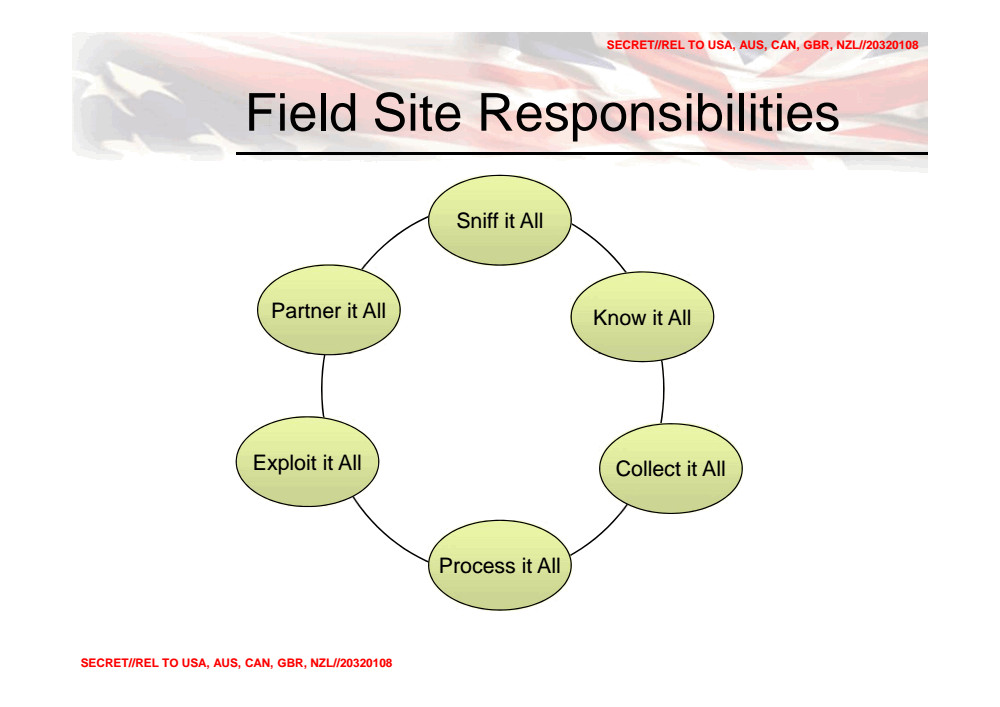
\includegraphics[scale=0.3]{pics/collect_it_all}
\end{frame}


\begin{frame}{Meta-data leakage}
  Encryption is NOT sufficient!
  \break
  
  Leaked meta-data:
  \begin{itemize}
  \item Geographical location
  \item Message sender
  \item Message receiver
  \item Message send time
  \item Message receive time
  \item Frequency of received messages
  \item Frequency of sent messages
  \item Size of the message
  \item Message sequence
  \end{itemize}
\end{frame}



\begin{frame}{anonymity options}
  \begin{itemize}
  \item decryption mix networks
  \item private information retrieval
  \item dining cryptographer networks
  \item broadcast based designs
  \item oblivious random access memory
  \item secure multi-party computation
  \item verified mix shuffles
  \end{itemize}
\end{frame}


\begin{frame}
\hspace*{3pt} David Chaum. {\em Untraceable electronic mail, return addresses, and \\
\hspace*{3pt} digital pseudonyms}, Comm. ACM, 24, 2 (Feb. 1981); 84-90
\break
\end{frame}

\begin{frame}
Chaum came up with many big ideas in this paper such as:
\begin{itemize}
  \item Sender anonymity
  \item Anonymous replies
  \item Message receipts for reliability
  \item Pseudonyms for persistent communication
  \end{itemize}
\end{frame}

\begin{frame}
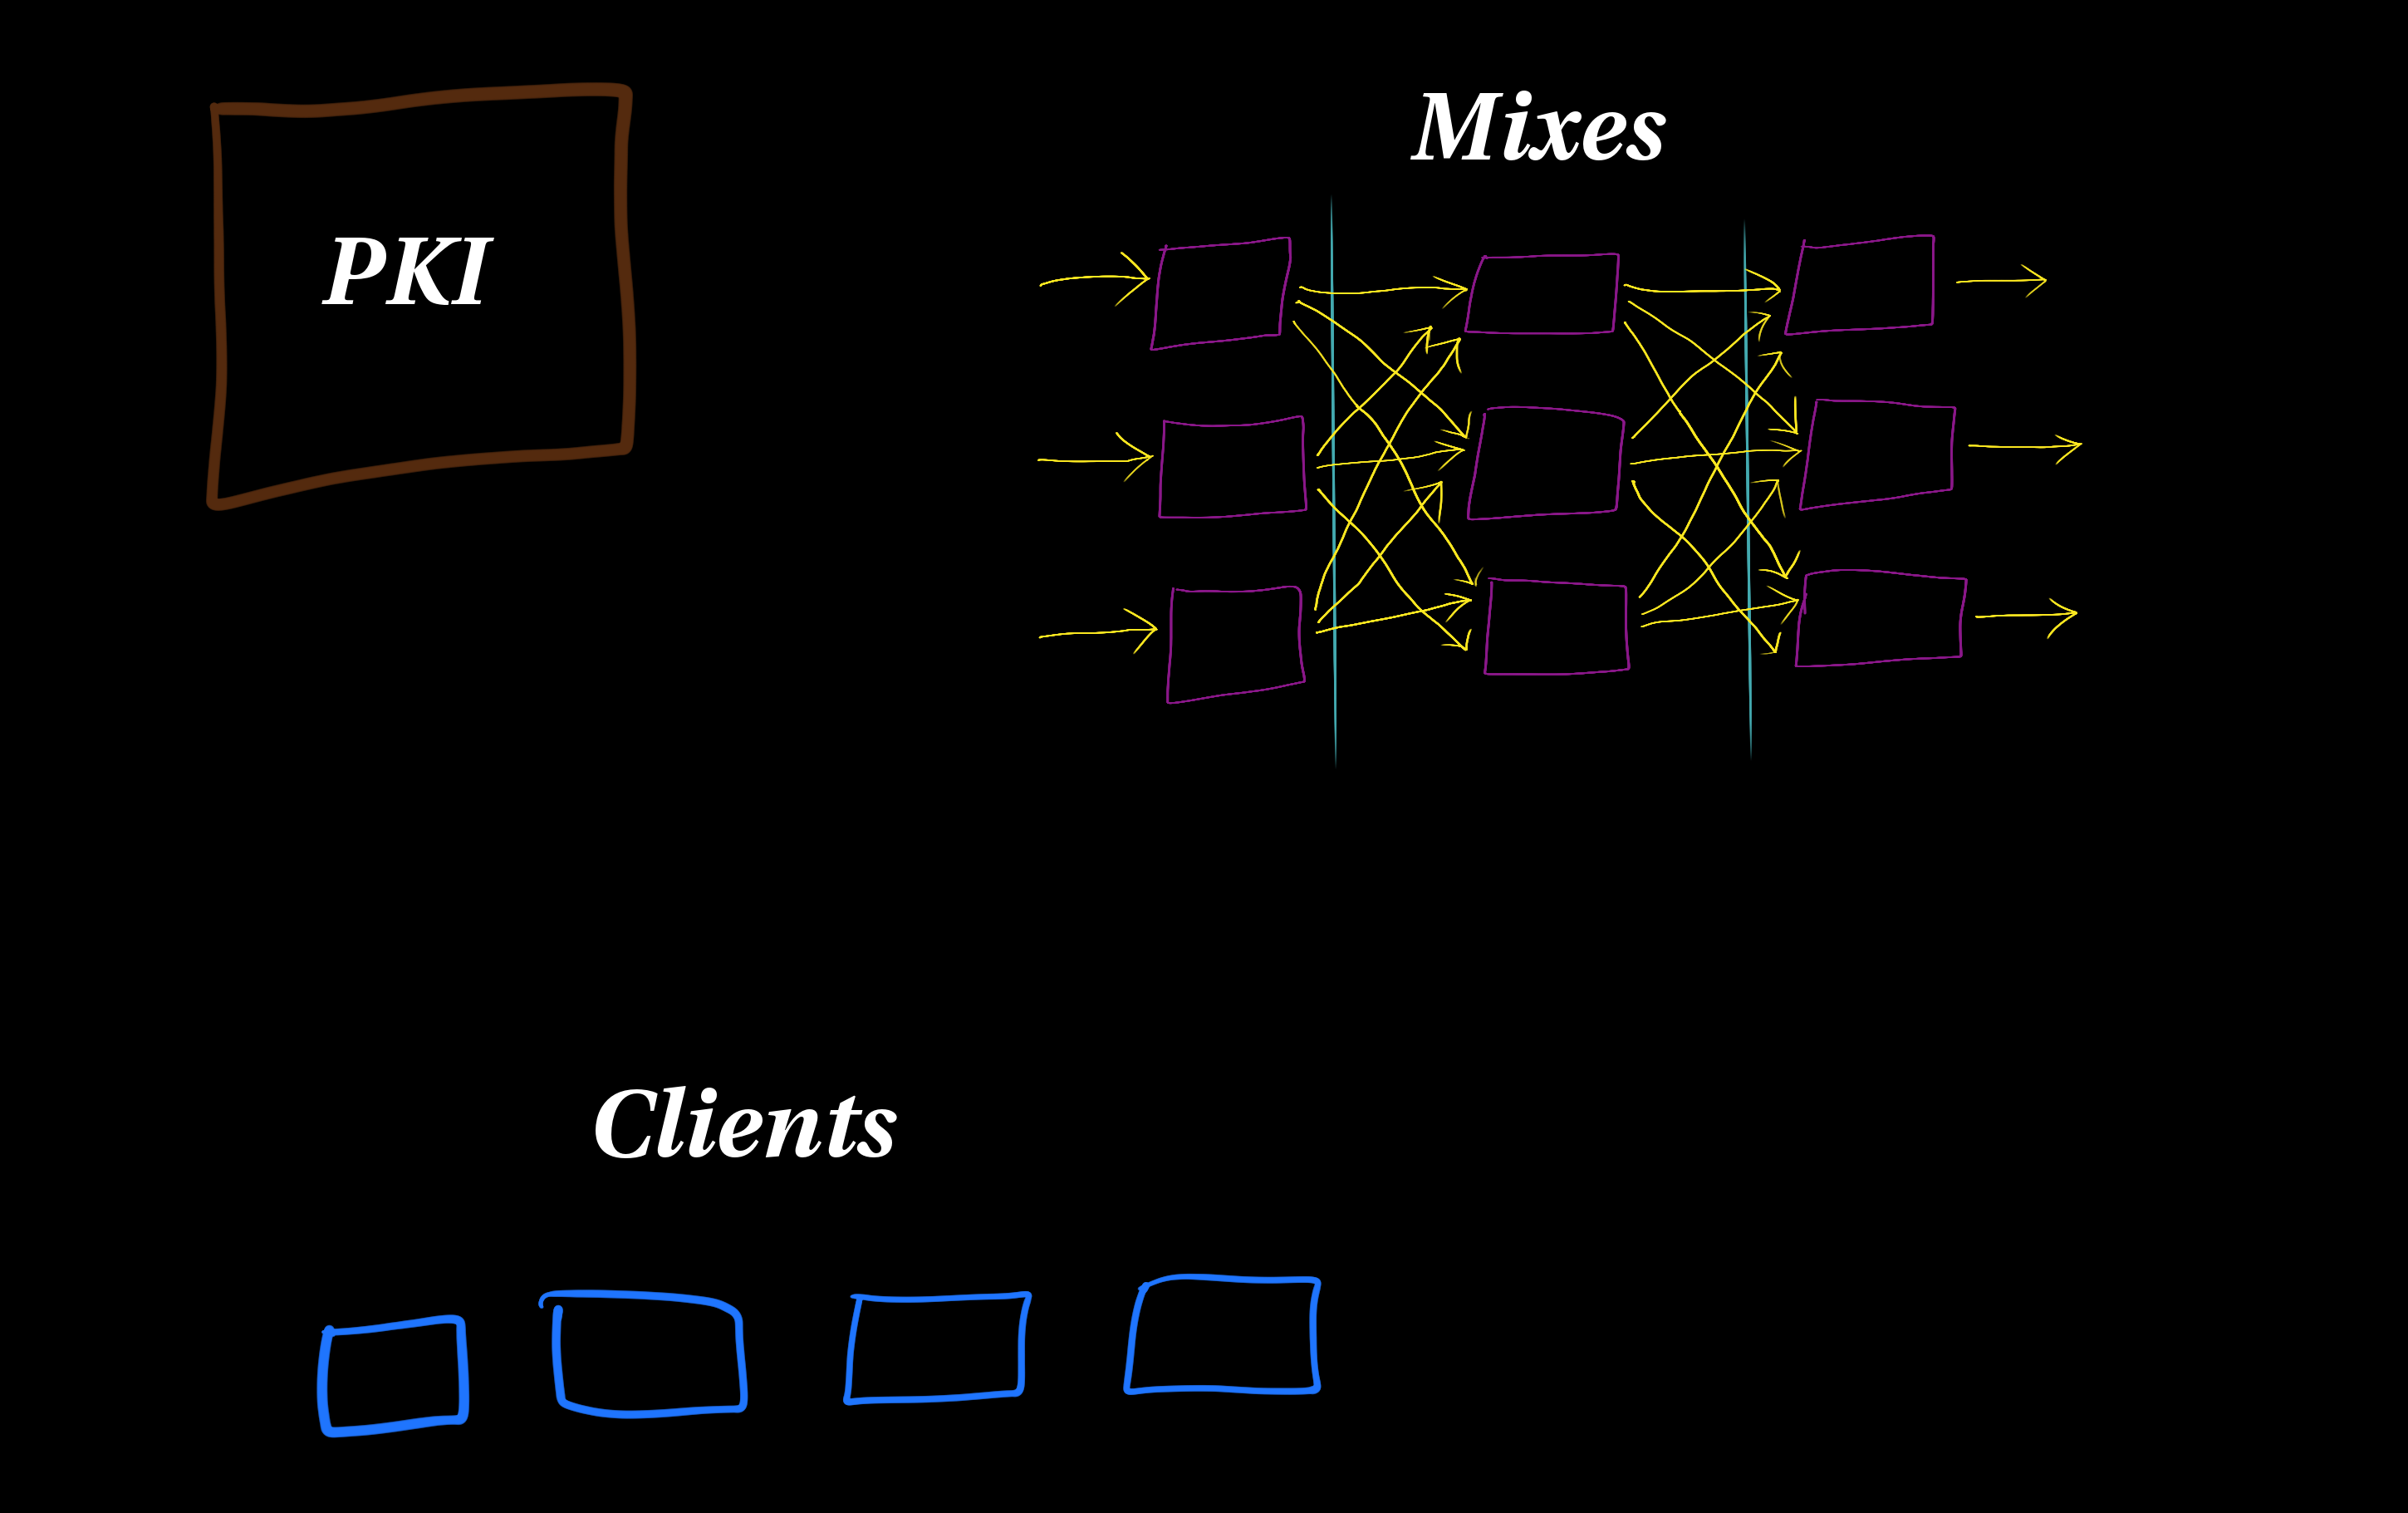
\includegraphics[scale=.10]{pics/mixnet_architecture1}
\end{frame}

\begin{frame}
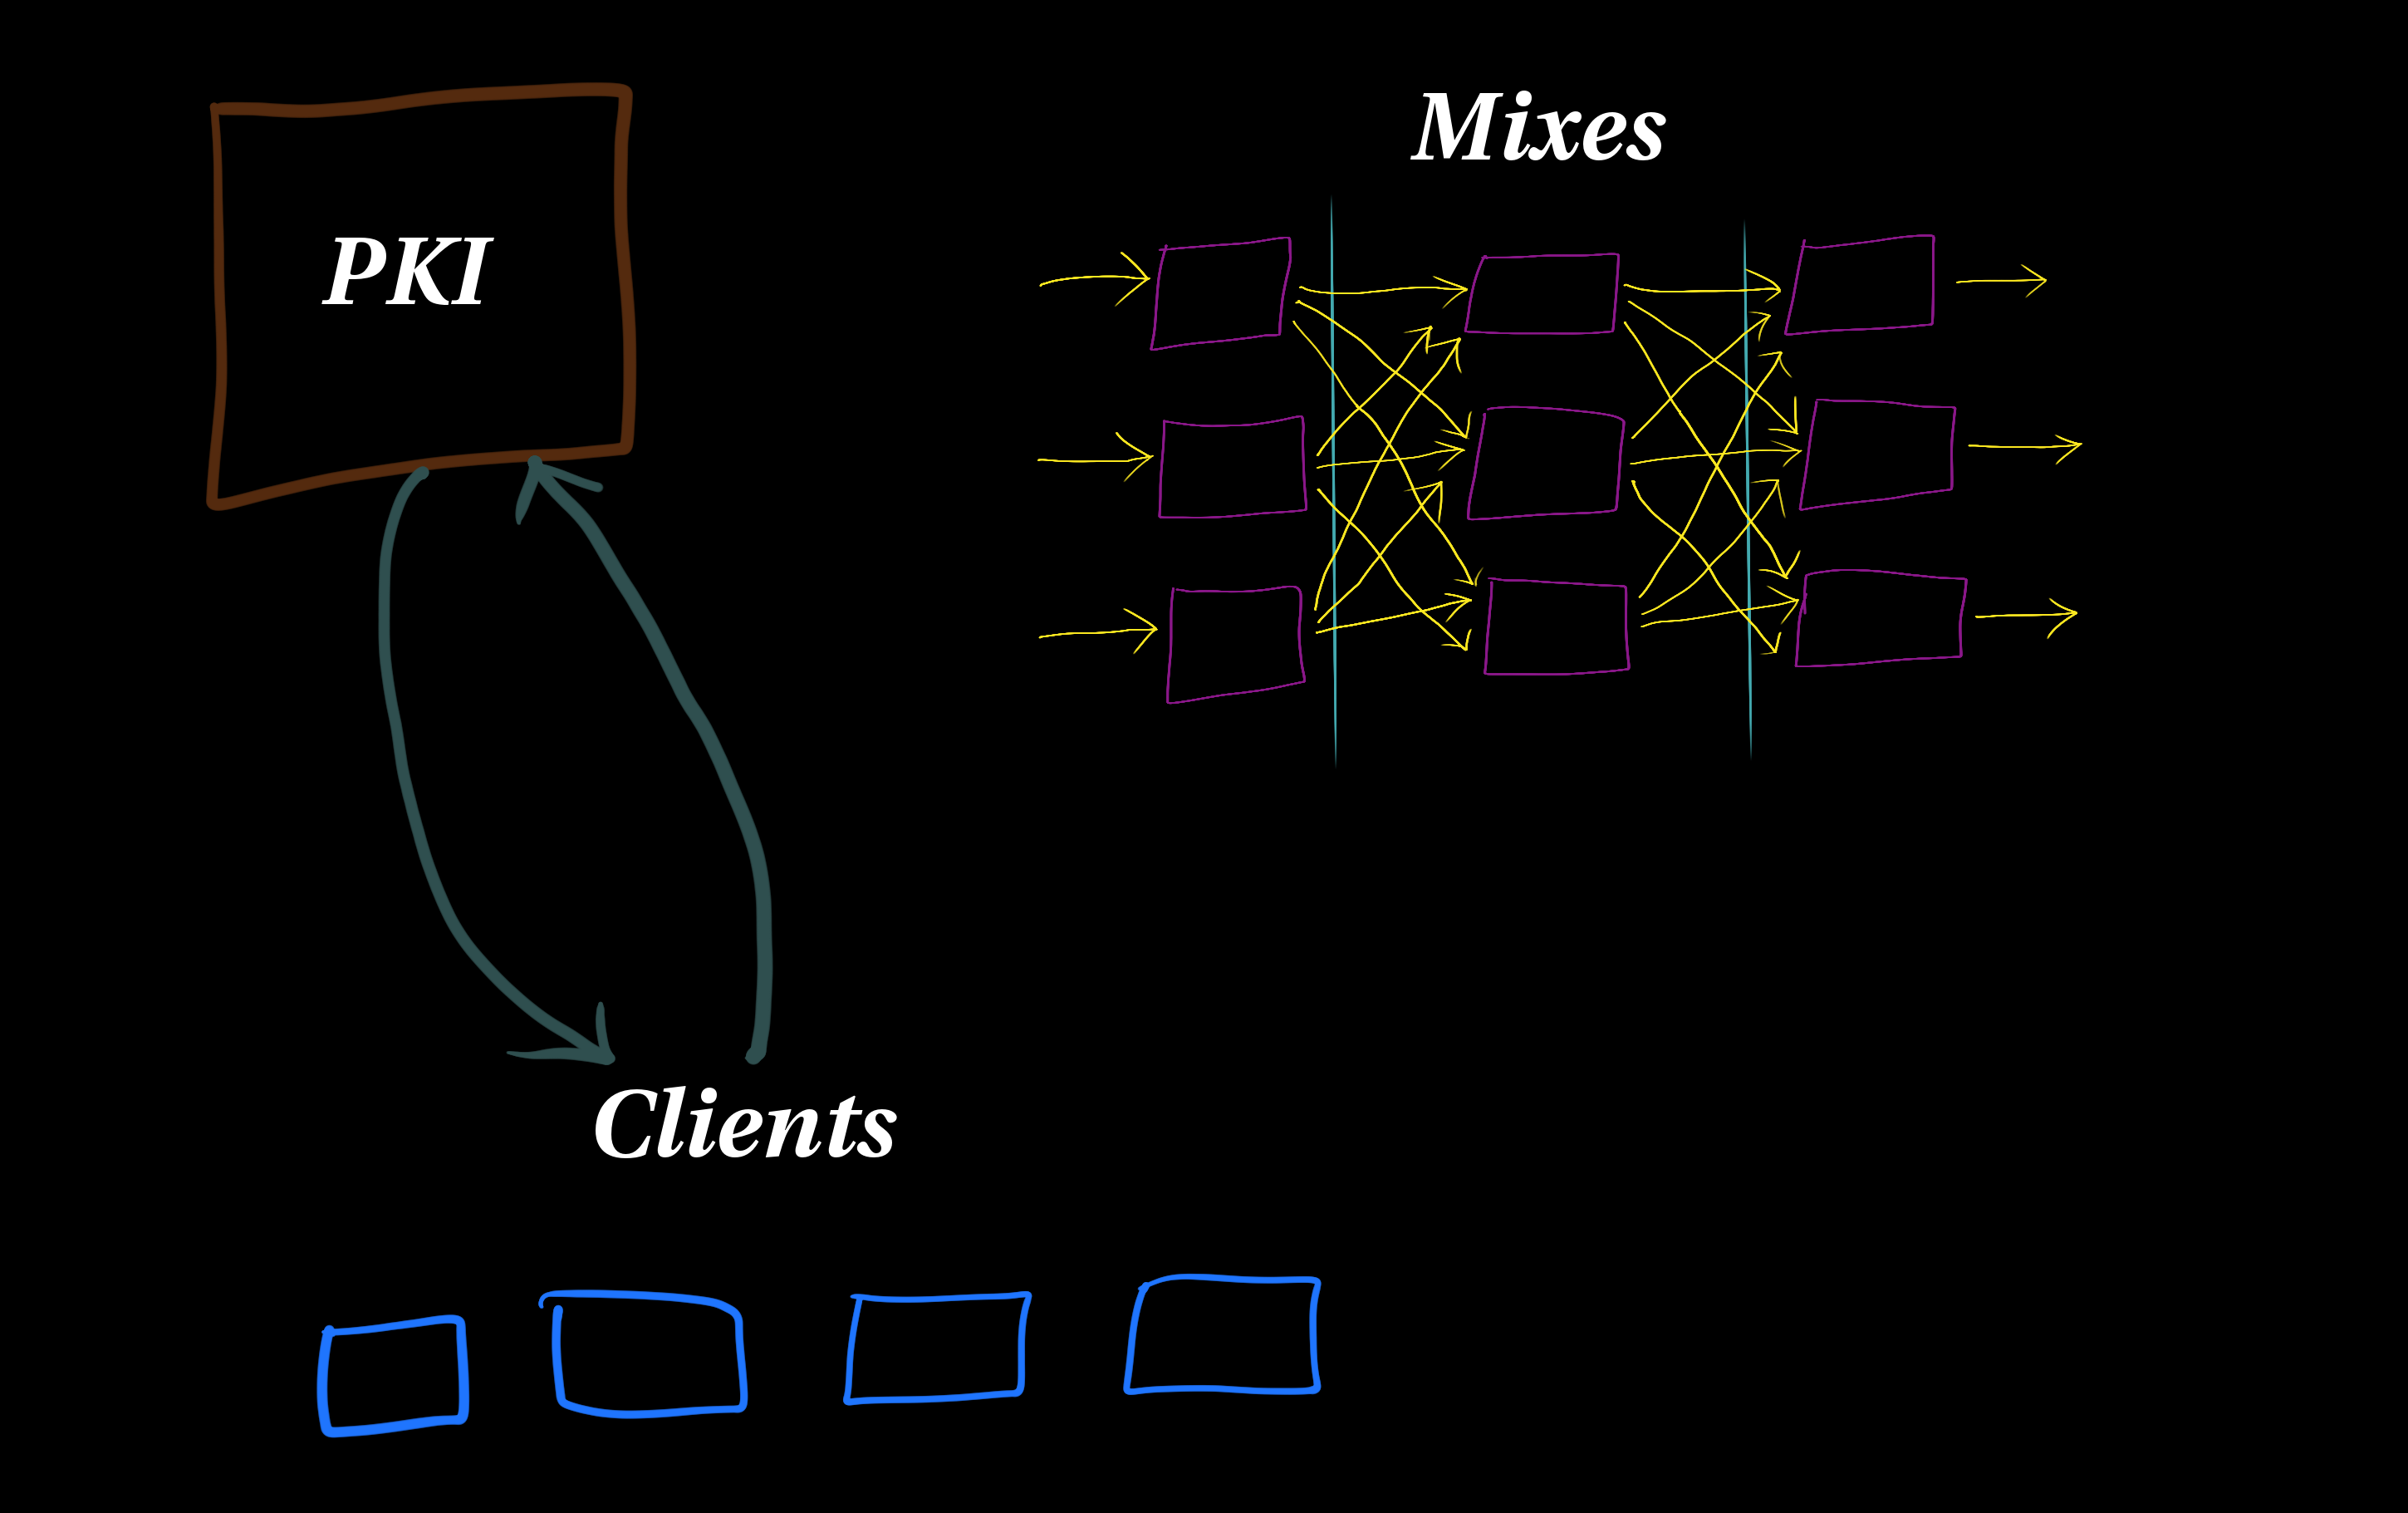
\includegraphics[scale=.10]{pics/mixnet_architecture2}
\end{frame}

\begin{frame}
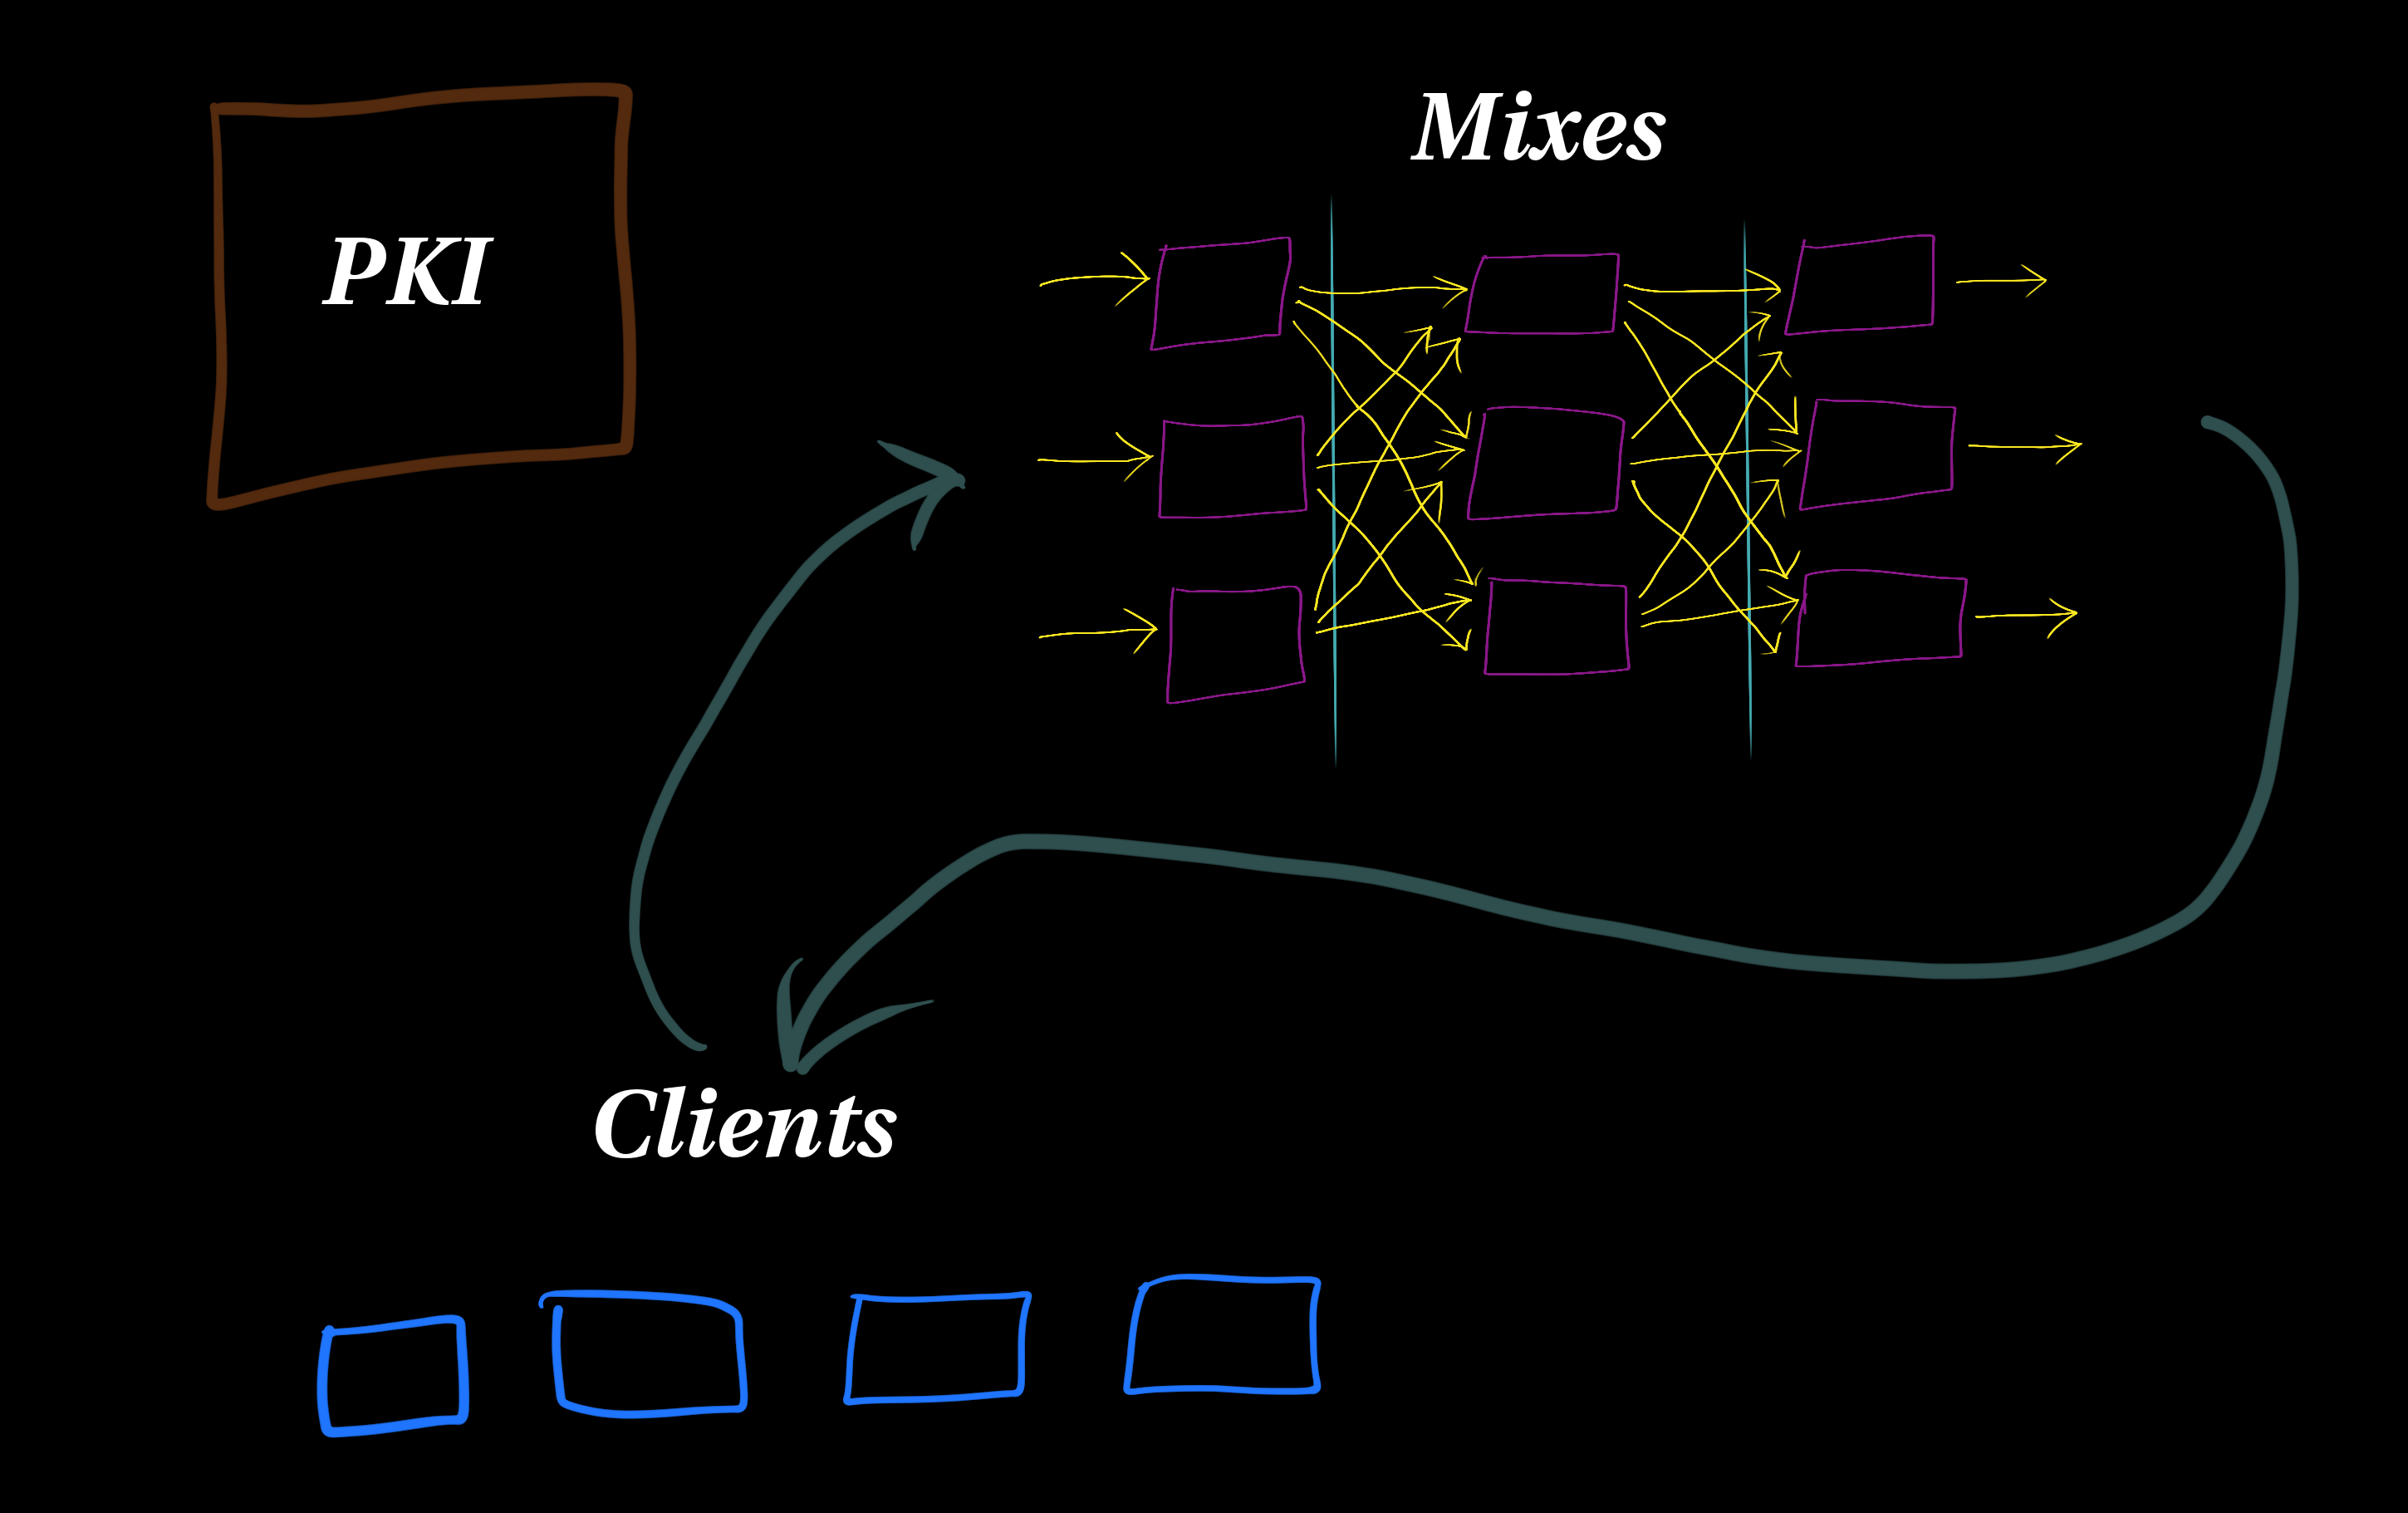
\includegraphics[scale=.10]{pics/mixnet_architecture3}
\end{frame}

\begin{frame}
\begin{center}
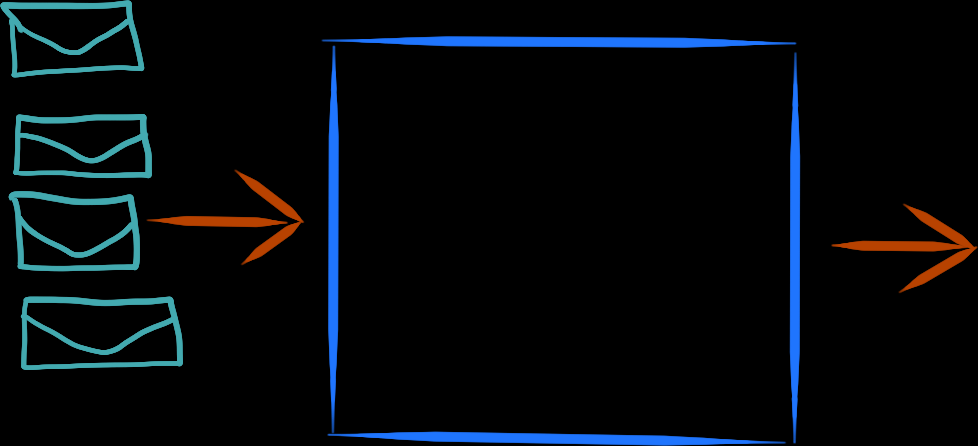
\includegraphics[scale=.20]{pics/mix1}
\end{center}
\end{frame}

\begin{frame}
\begin{center}
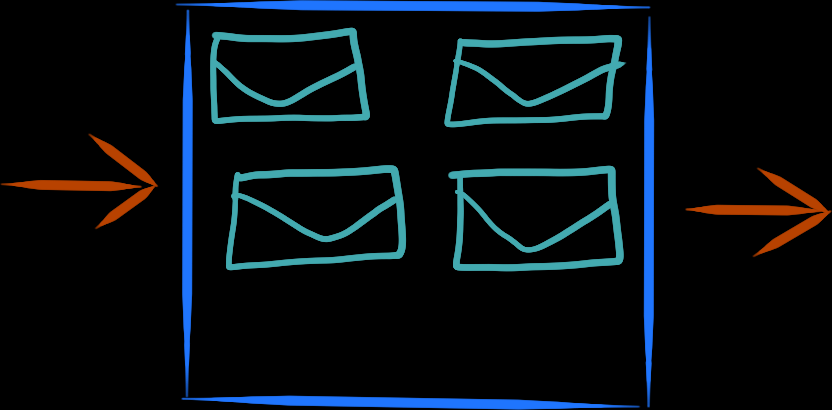
\includegraphics[scale=.20]{pics/mix2}
\end{center}
\end{frame}

\begin{frame}
\begin{center}
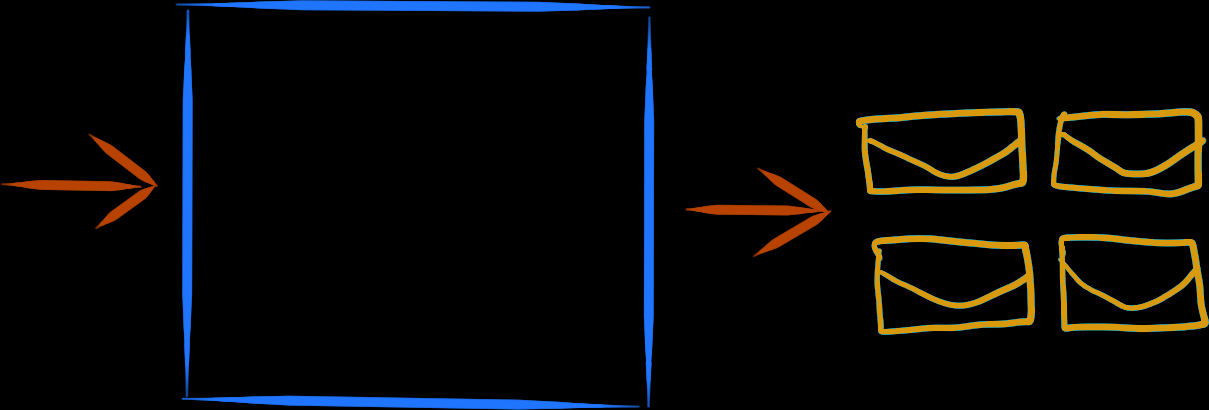
\includegraphics[scale=.20]{pics/mix3}
\end{center}
\end{frame}

\begin{frame}
\bigskip

See: \\ \smallskip

\hspace*{3pt} Claudia Diaz \& Andrei Serjantov.  {\em Generalising Mixes.}  PETS 2003
\end{frame}


\begin{frame}
\begin{center}
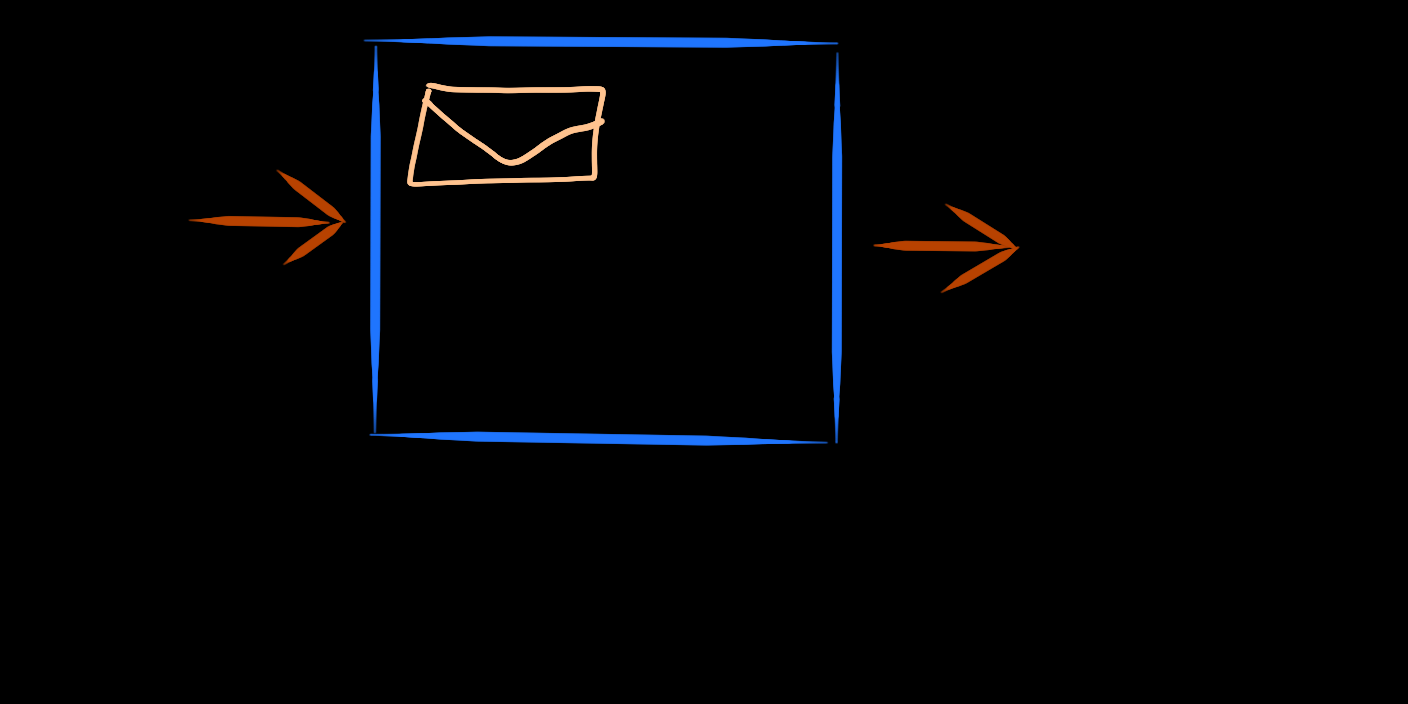
\includegraphics[scale=.23]{pics/blending1}
\end{center}
\end{frame}

\begin{frame}
\begin{center}
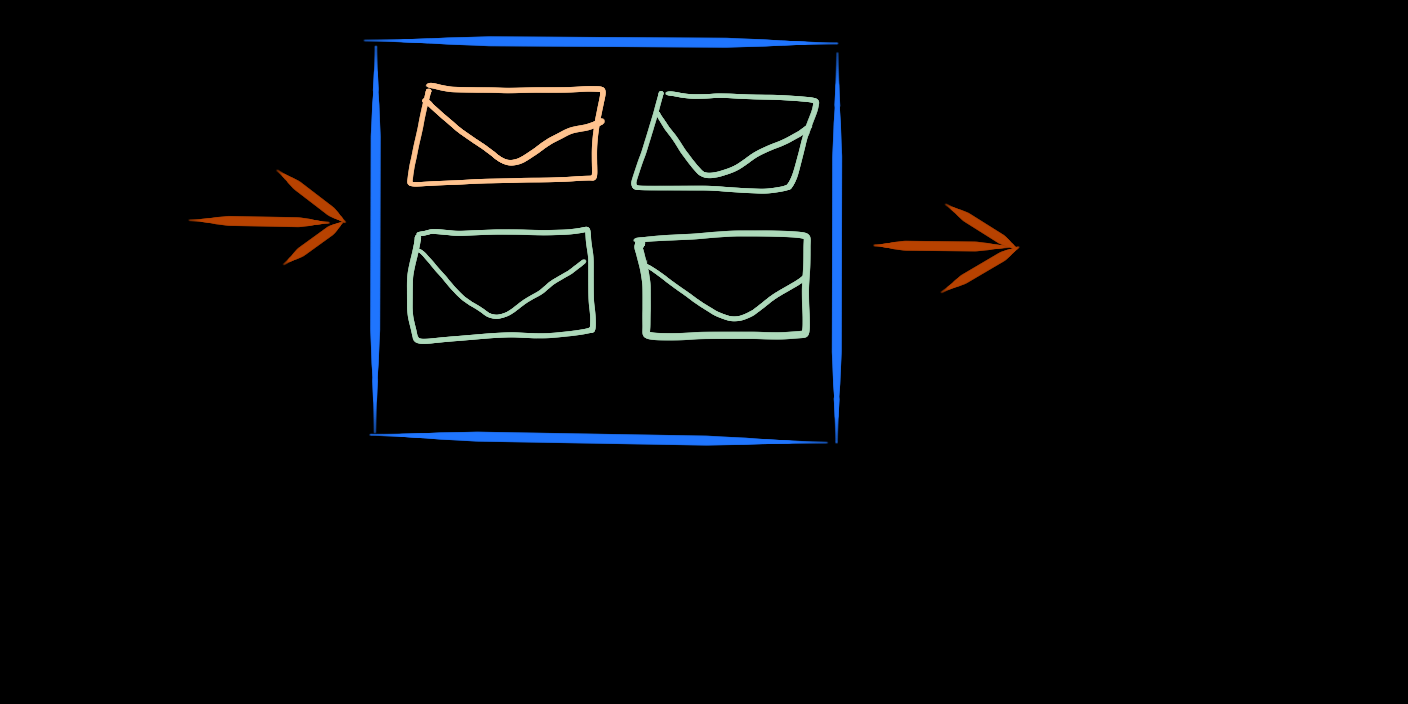
\includegraphics[scale=.23]{pics/blending2}
\end{center}
\end{frame}

\begin{frame}
\begin{center}
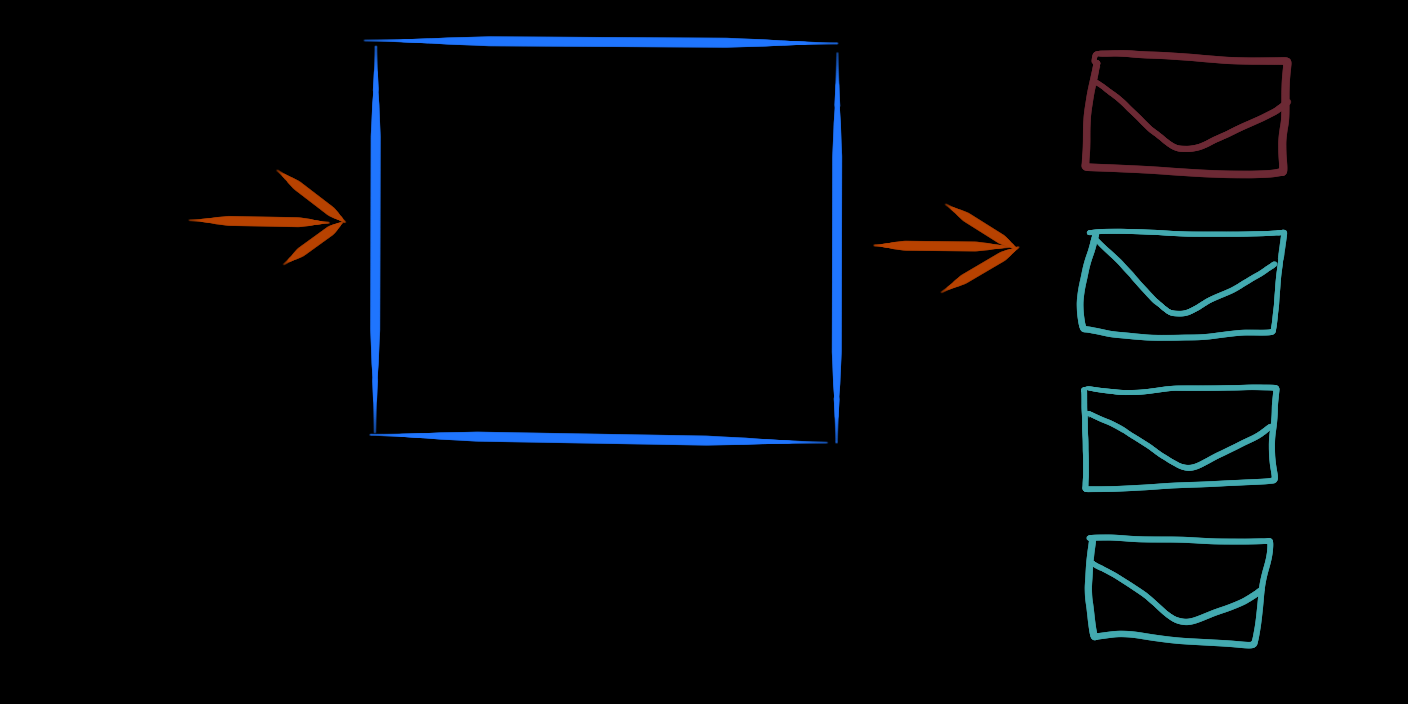
\includegraphics[scale=.23]{pics/blending3}
\end{center}
\end{frame}



\begin{frame}
\begin{center}
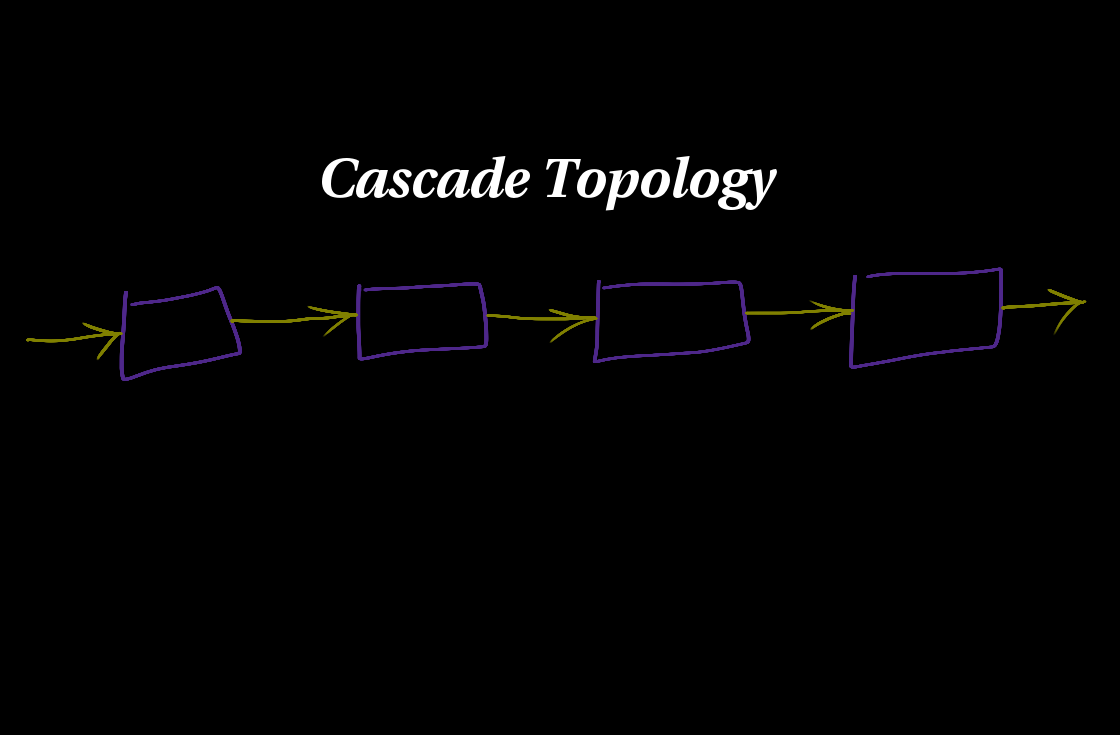
\includegraphics[scale=.30]{pics/cascade}
\end{center}
\end{frame}

\begin{frame}
\begin{center}
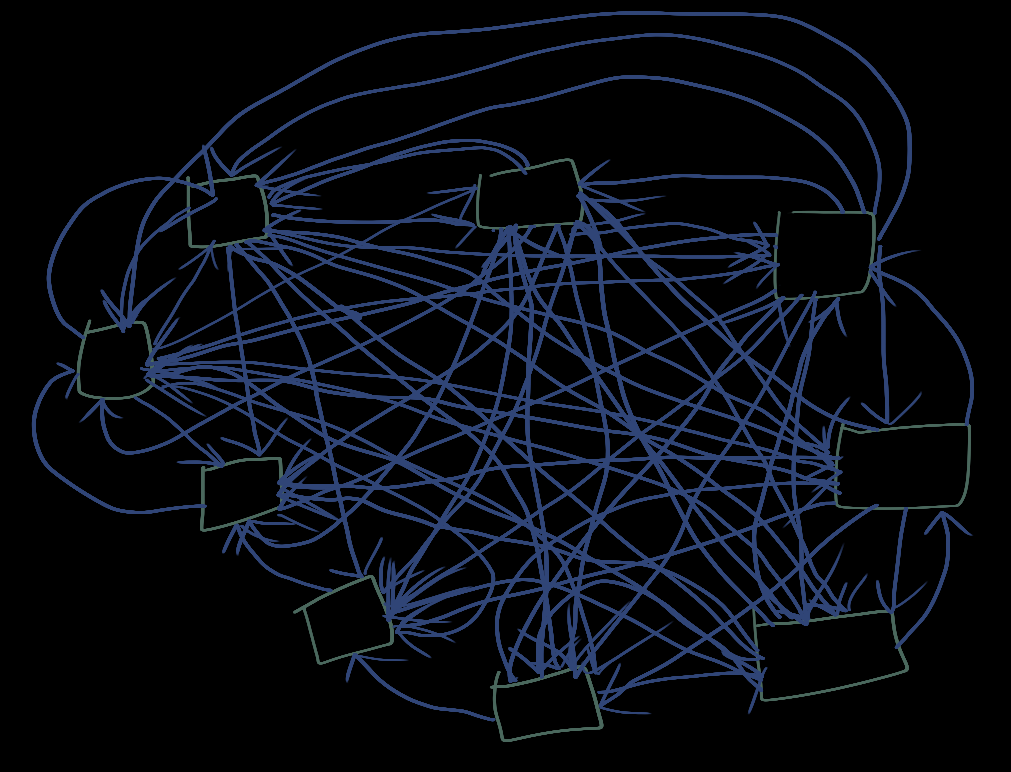
\includegraphics[scale=.30]{pics/free_route1}
\end{center}
\end{frame}

\begin{frame}
\begin{center}
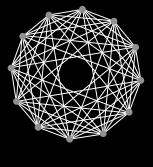
\includegraphics[scale=1]{pics/free_route2}
\end{center}
\end{frame}

\begin{frame}
\begin{center}
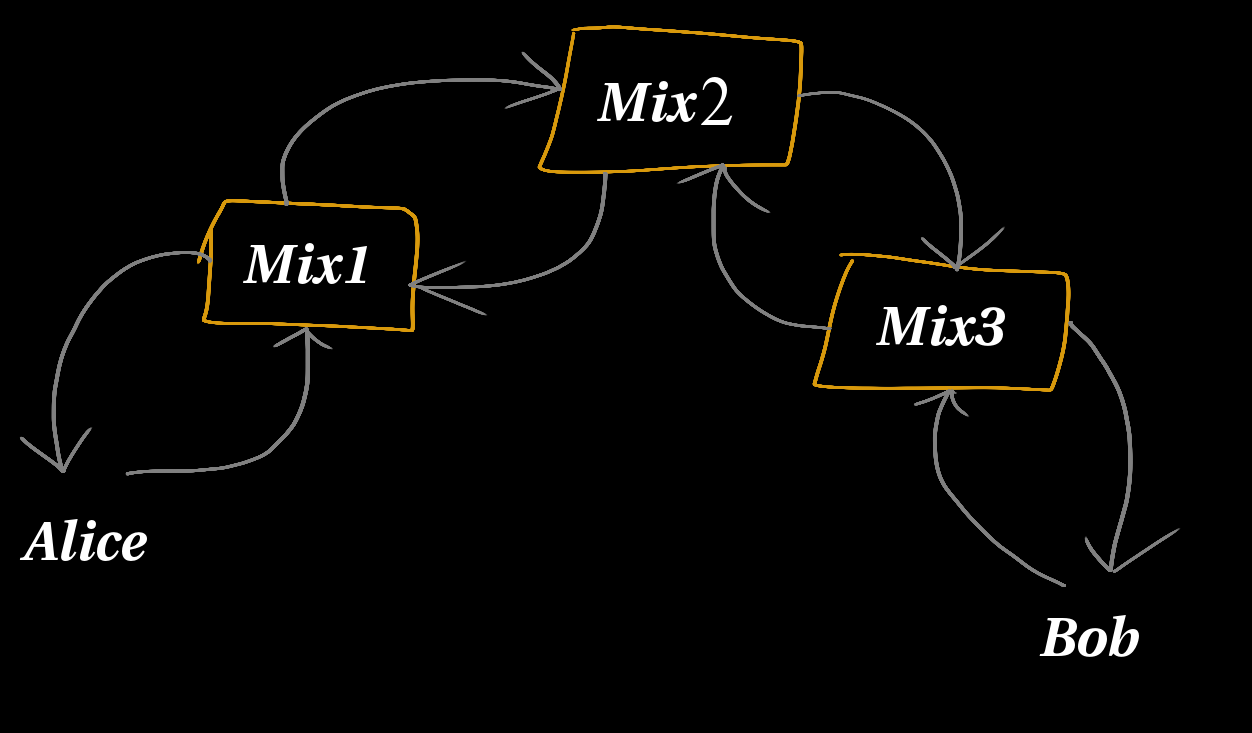
\includegraphics[scale=.25]{pics/free_route3}
\end{center}
\end{frame}

\begin{frame}
\begin{center}
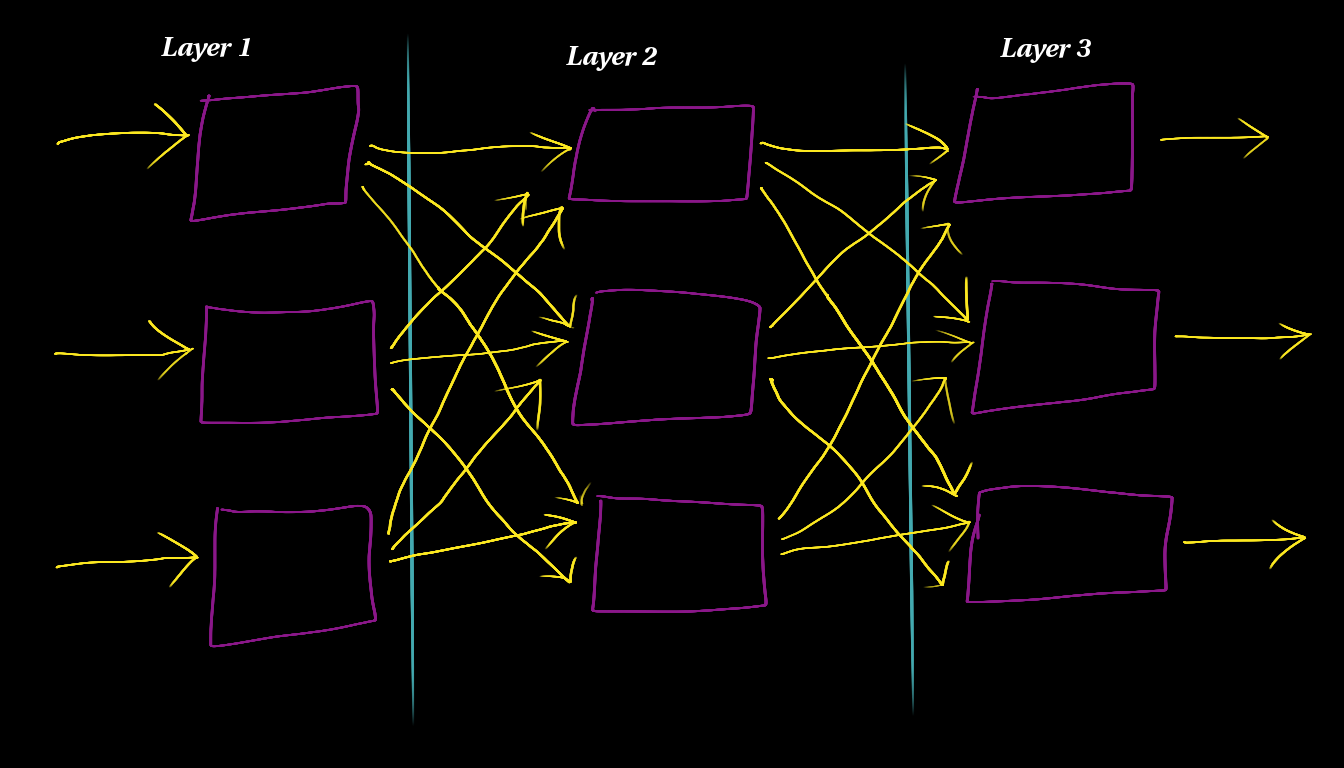
\includegraphics[scale=.24]{pics/stratified_topology1}
\end{center}
\end{frame}

\begin{frame}
\begin{center}
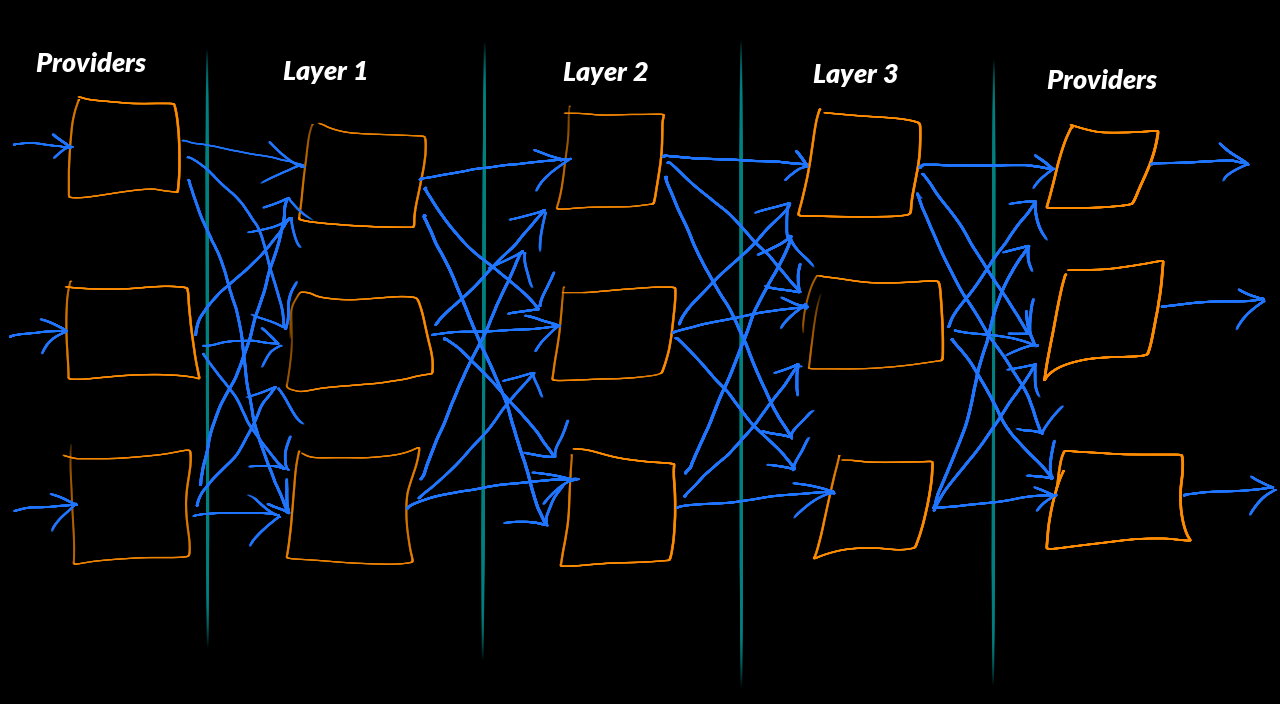
\includegraphics[scale=.25]{pics/stratified_topology2}
\end{center}
\end{frame}

\begin{frame}
\begin{center}
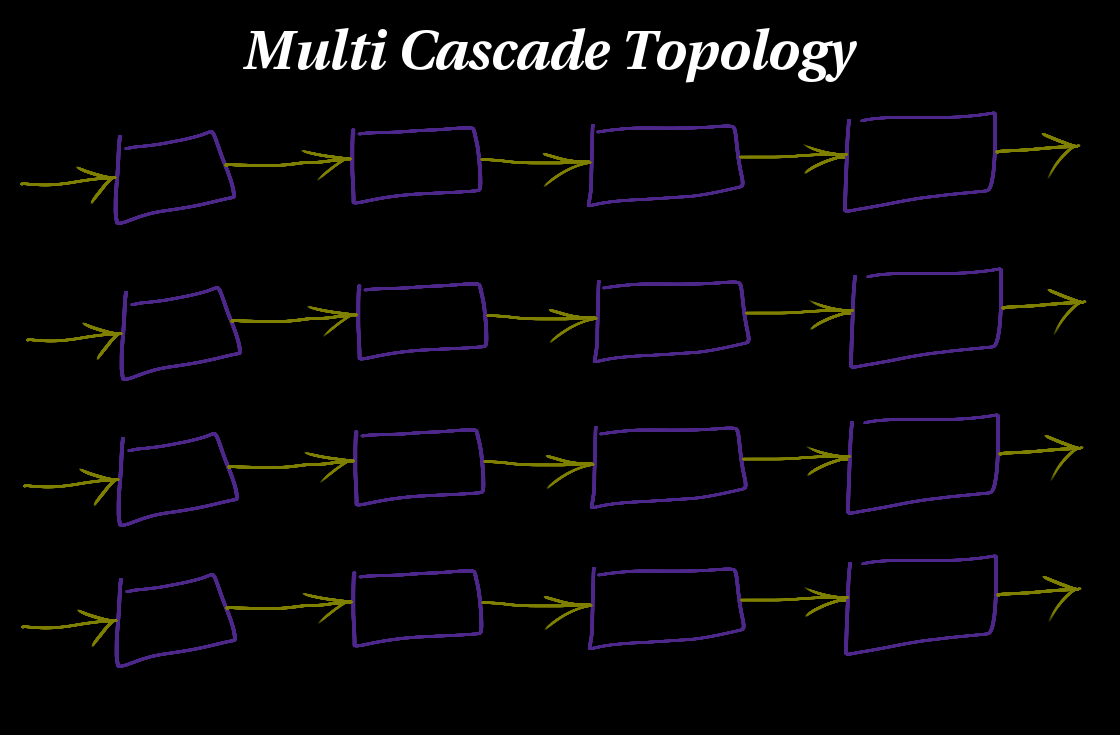
\includegraphics[scale=.29]{pics/multi_cascade}
\end{center}
\end{frame}


\begin{frame}
\hspace*{3pt} Diaz, Murdoch, Troncoso.  {\em Impact of Network Topology on \\
\hspace*{3pt} Anonymity and Overhead in Low-Latency Anonymity Networks} \\
\hspace*{3pt} PETs 2010
\end{frame}


\begin{frame}
\begin{center}
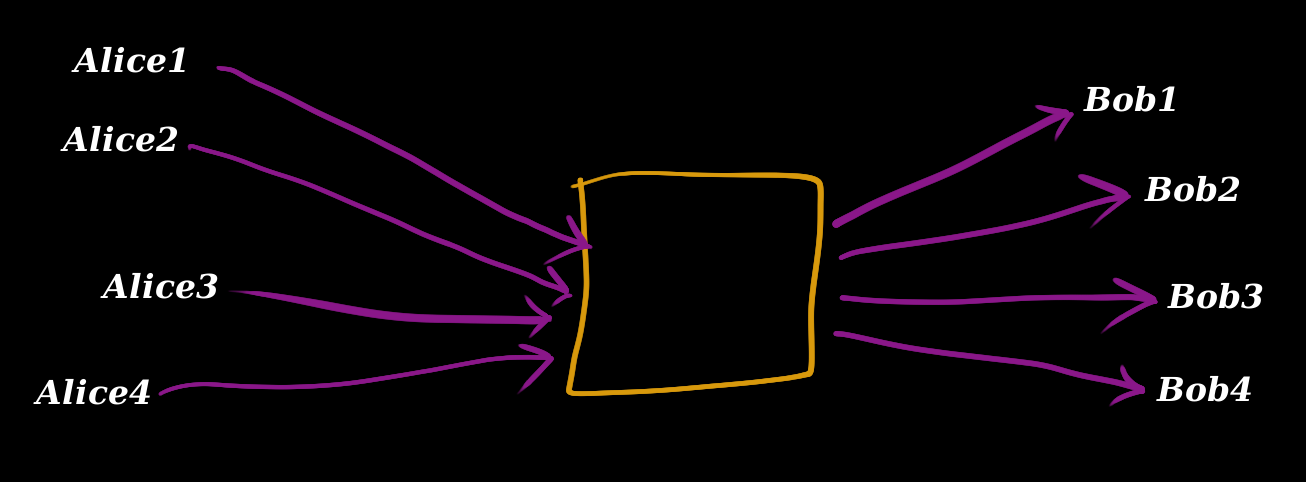
\includegraphics[scale=.24]{pics/sda1}
\end{center}
\end{frame}

\begin{frame}
\begin{center}
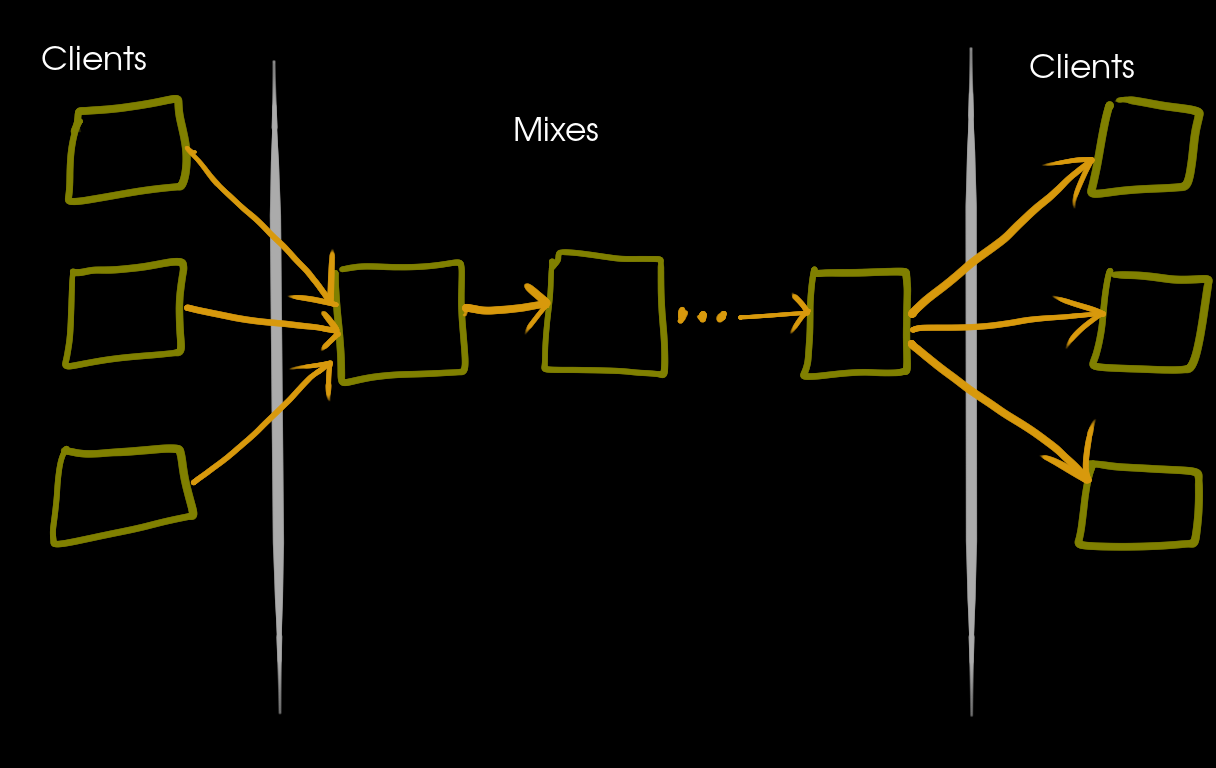
\includegraphics[scale=.26]{pics/sda2}
\end{center}
\end{frame}

\begin{frame}
\begin{center}
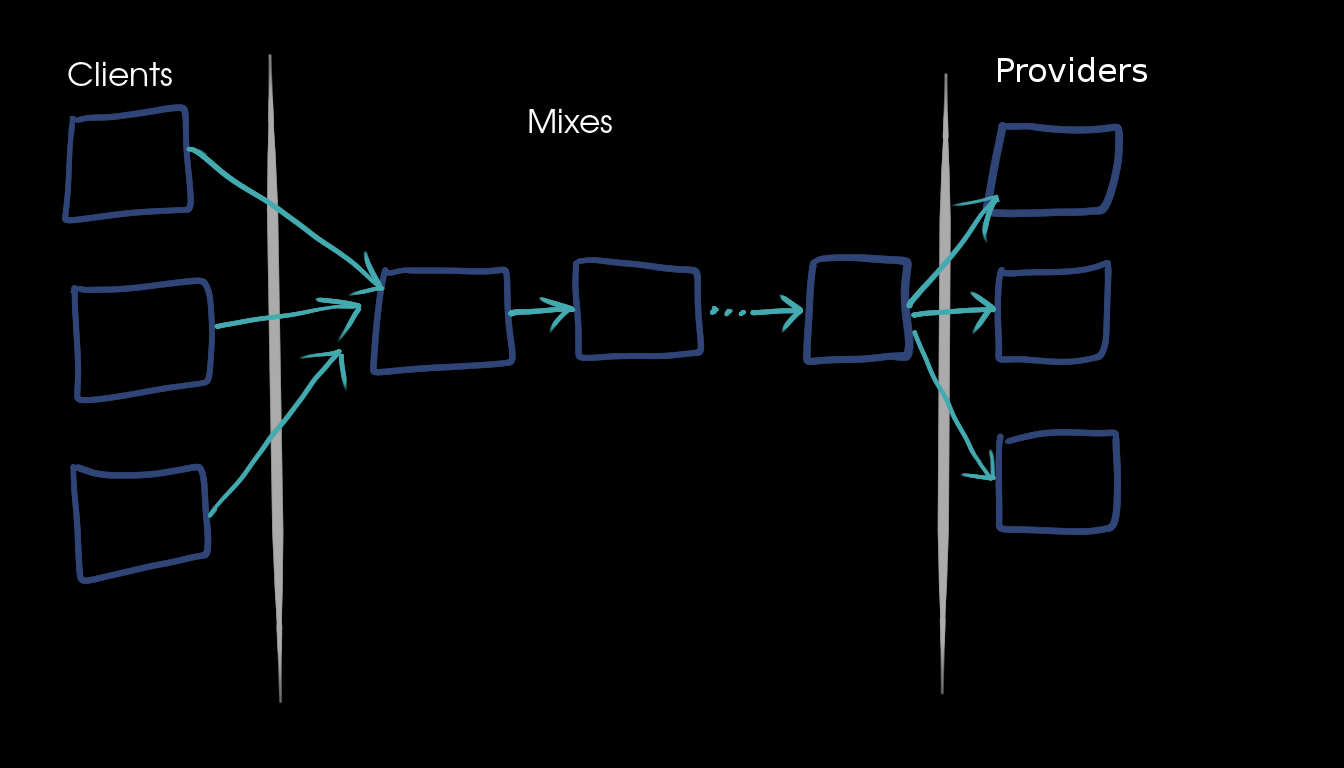
\includegraphics[scale=.24]{pics/sda3}
\end{center}
\end{frame}

\begin{frame}
\begin{center}
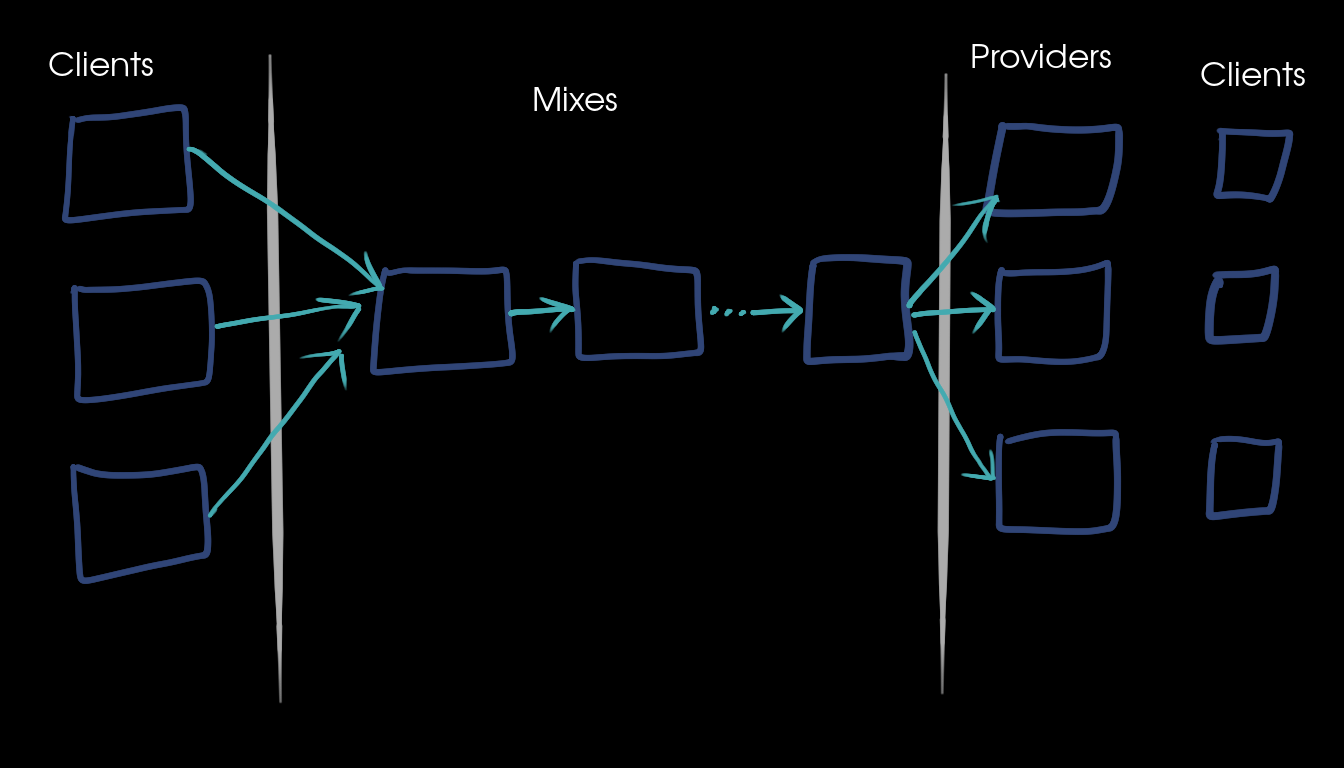
\includegraphics[scale=.24]{pics/sda4}
\end{center}
\end{frame}

\begin{frame}
\begin{center}
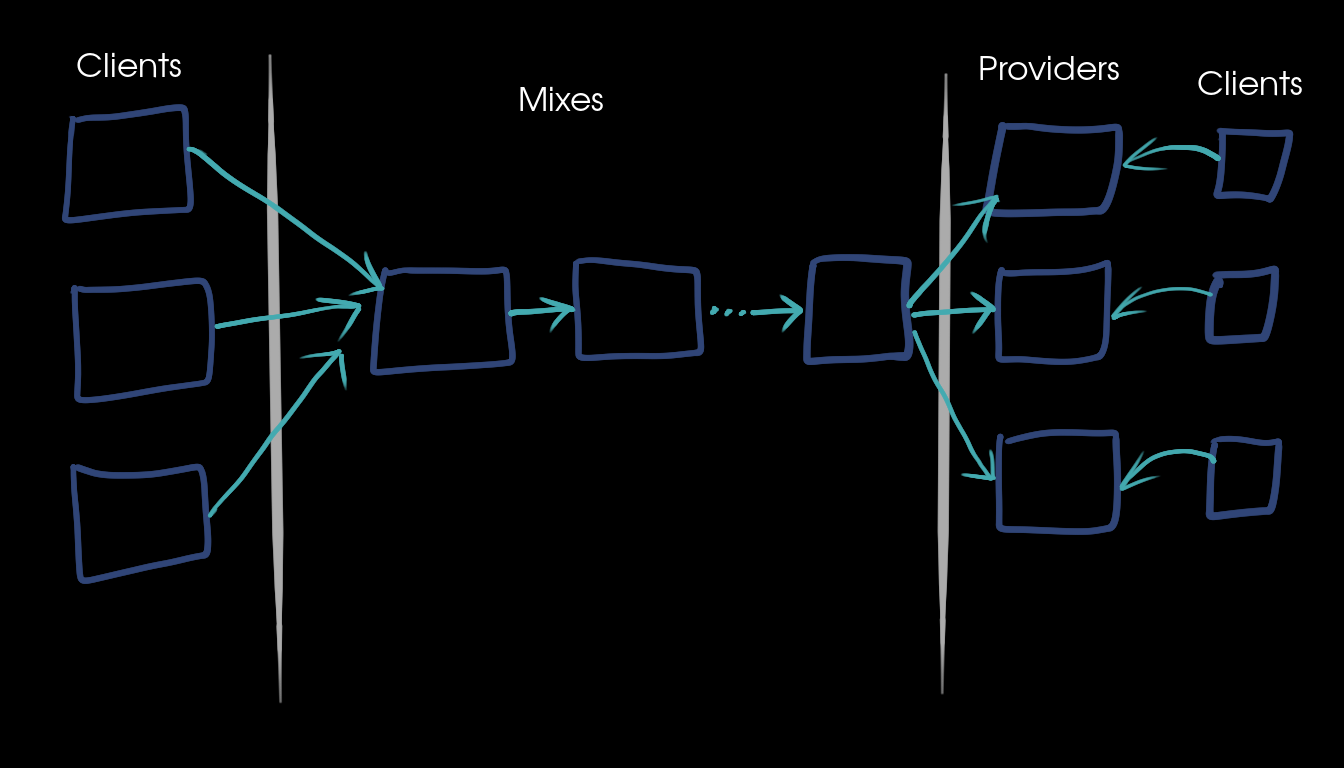
\includegraphics[scale=.24]{pics/sda5}
\end{center}
\end{frame}

\begin{frame}
\begin{center}
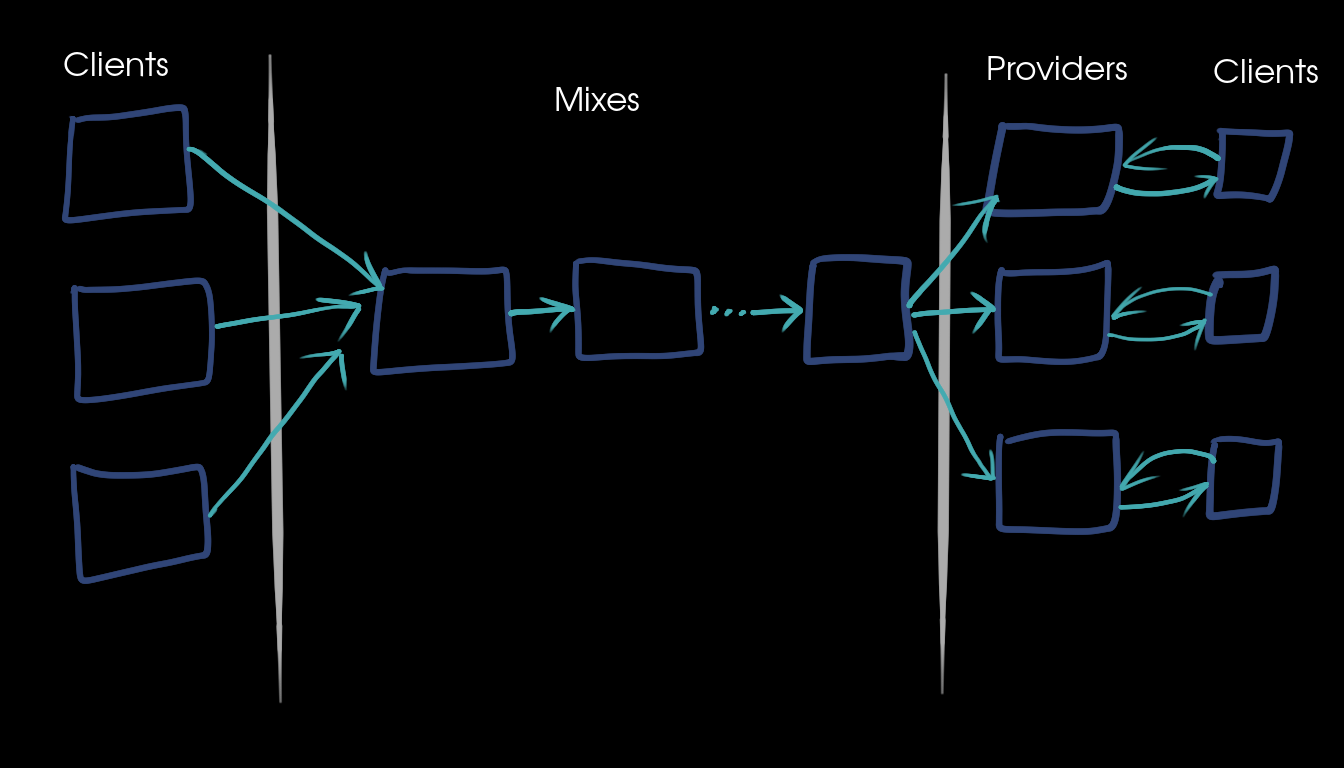
\includegraphics[scale=.24]{pics/sda6}
\end{center}
\end{frame}

\begin{frame}
\begin{center}
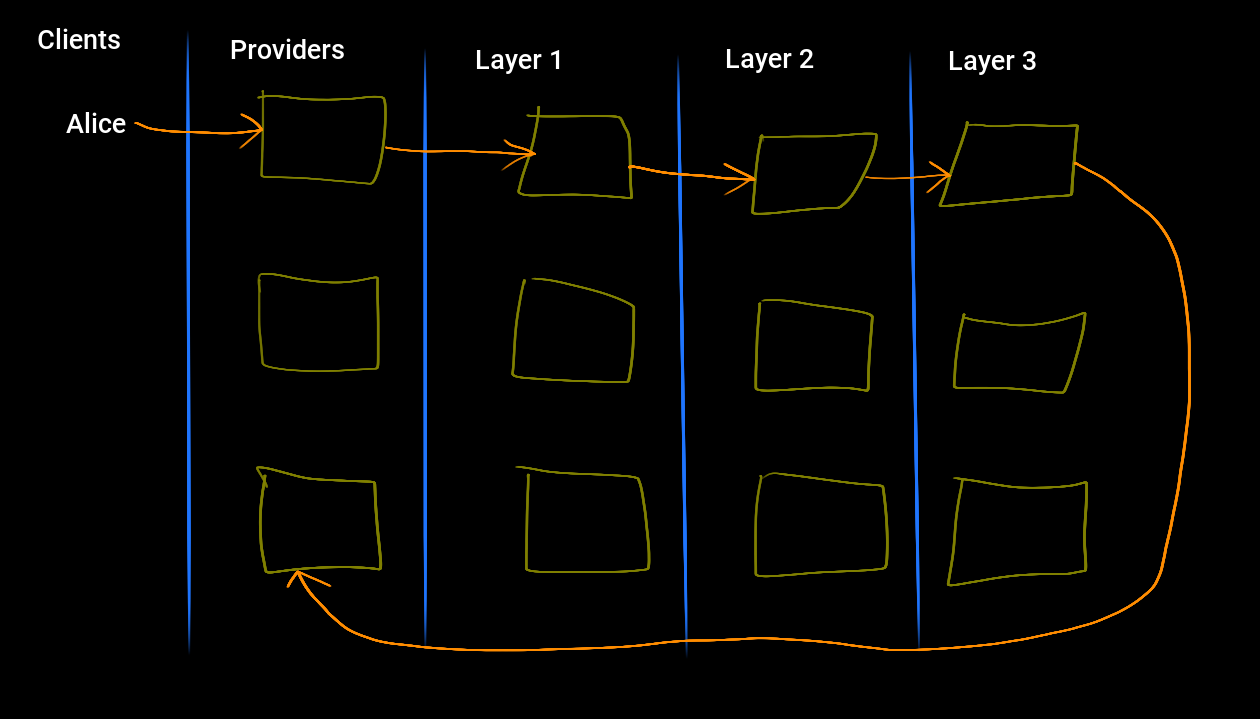
\includegraphics[scale=.24]{pics/katzenpost_loop1}
\end{center}
\end{frame}

\begin{frame}
\begin{center}
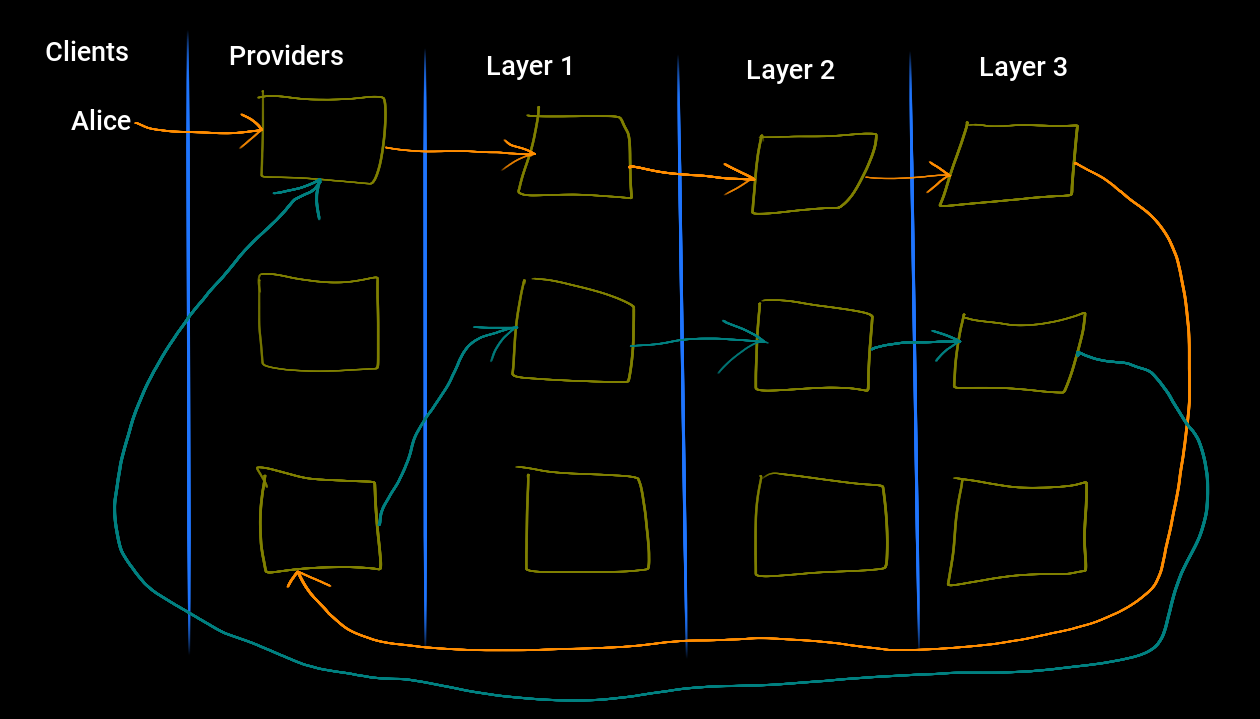
\includegraphics[scale=.24]{pics/katzenpost_loop2}
\end{center}
\end{frame}

\begin{frame}
\begin{center}
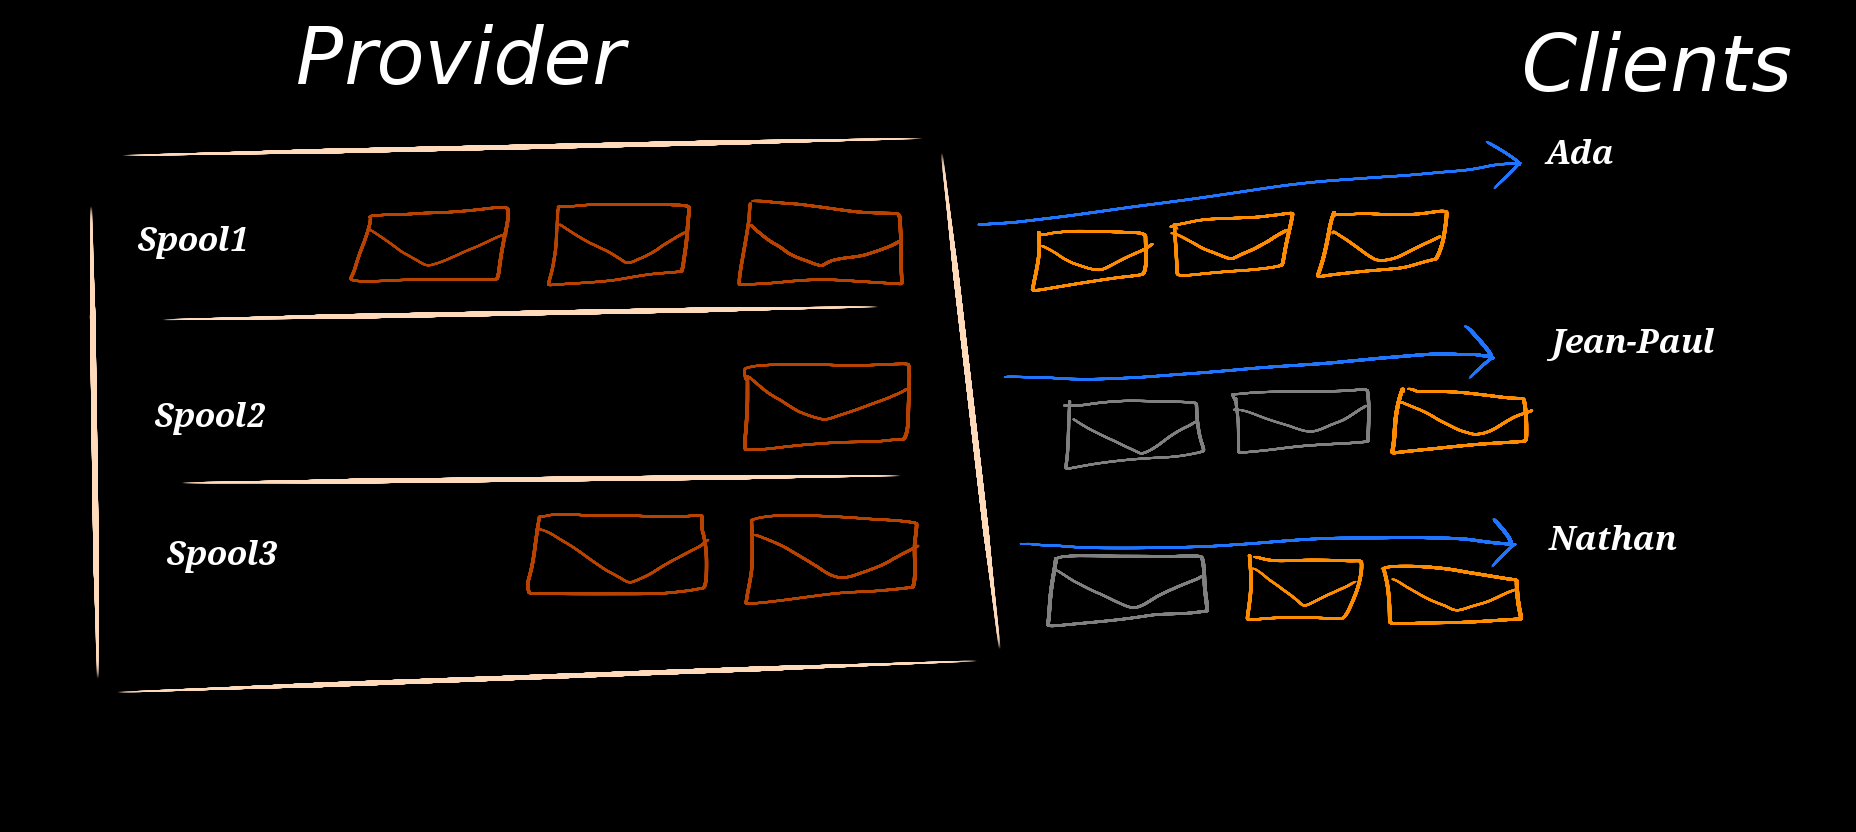
\includegraphics[scale=.18]{pics/provider_spools}
\end{center}
\end{frame}

\begin{frame}{Don't roll your own cryptographic packet format!}
"Sphinx: A Compact and Provably Secure Mix Format"  
by George Danezis and Ian Goldberg.
\end{frame}

\begin{frame}{Sphinx features}
  \begin{itemize}
  \item per hop bitwise unlinkability
  \item Single Use Reply Blocks
  \item indistinguishable replies
  \item hidden path length
  \item hidden relay position
  \item tagging attack detection
  \item replay attack detection
  \end{itemize}    
\end{frame}

\begin{frame}
\begin{center}
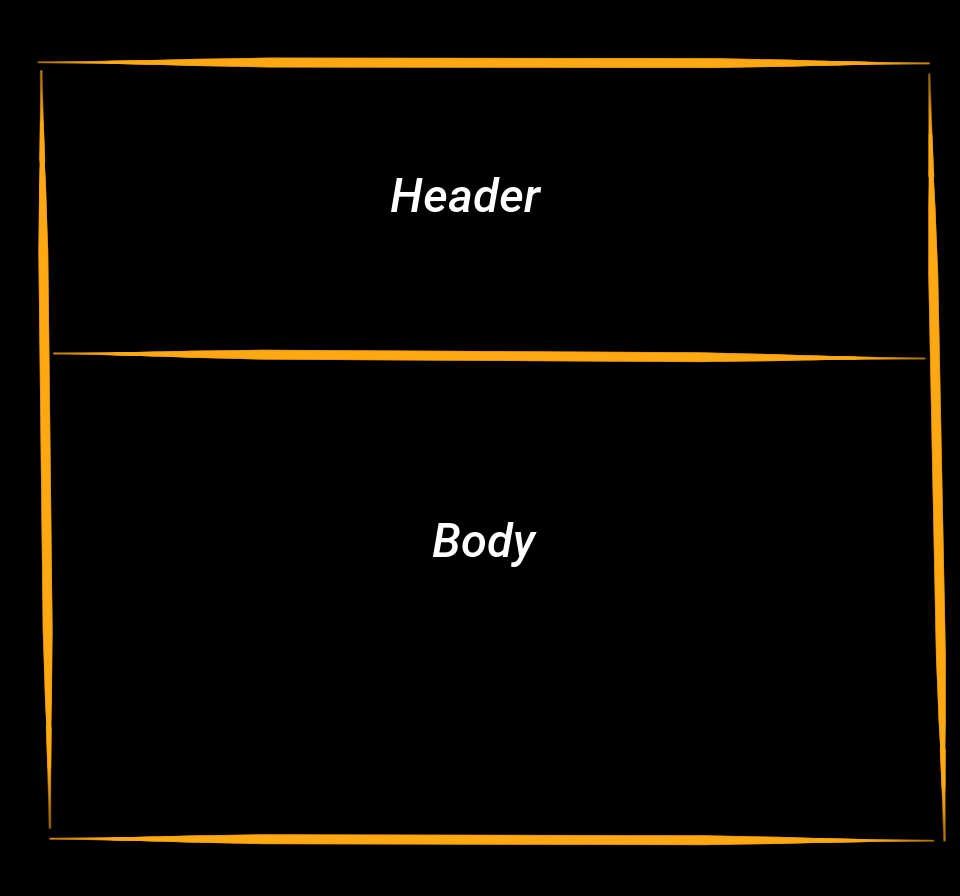
\includegraphics[scale=.27]{pics/sphinx1}
\end{center}
\end{frame}

\begin{frame}
\begin{center}
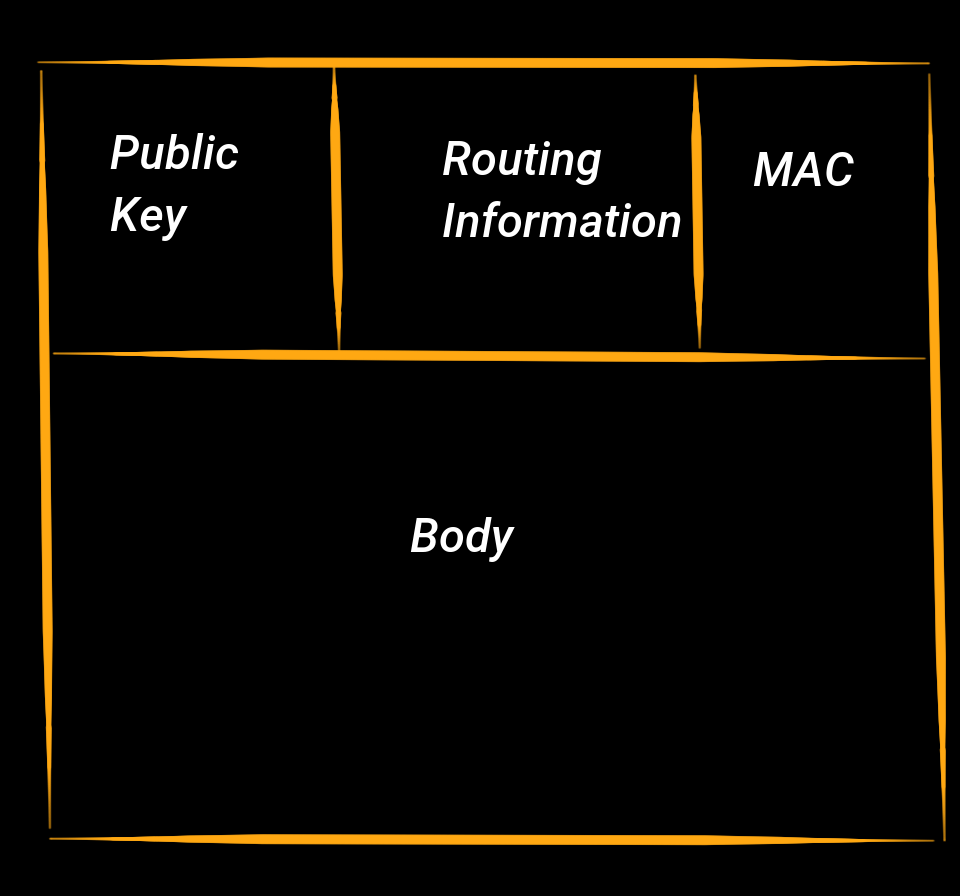
\includegraphics[scale=.27]{pics/sphinx2}
\end{center}
\end{frame}

\begin{frame}{Compulsion Attacks}
\begin{center}
  \vspace{5mm}
  \begin{itemize}
  \item legal action
  \item police raid
  \item pwn
  \end{itemize}  
\end{center}
\end{frame}

\begin{frame}{Compulsion Attacks Defenses via Mix Key Erasure}
\begin{center}
  \begin{itemize}
  \item Mix key rotation
  \item Forward secure mixes
  \end{itemize}  
\end{center}

\vspace{10mm}
``Forward Secure Mixes'' by George Danezis,
Proceedings of 7th Nordic Workshop on Secure IT Systems, 2002\\
\vspace{5mm}
``Xolotl: A request-and-forward mixnet format with selective statefulness for forward
secure and hybrid post-quantum anonymity'' by Jeffrey Burdges and Christian Grothoff

\end{frame}

\begin{frame}{Other Defenses for Compulsion Attacks}
\begin{center}
  \begin{itemize}
  \item multicast routing hops
  \item compulsion traps
  \item plausibly deniable routing
  \end{itemize}  
\end{center}

\vspace{5mm} %5mm vertical space

"Compulsion Resistant Anonymous Communications" by George Danezis and Jolyon Clulow,
Proceedings of Information Hiding Workshop, June 2005
\end{frame}


\begin{frame}{Other Considerations for Compulsion Attacks}
\vspace{5mm} %5mm vertical space
``No right to ramain silent: Isolating Malicious Mixes''
by Hemi Leibowitz, Ania Piotrowska, George Danezis and Amir Herzberg\\
\vspace{10mm}
``Two Cents for Strong Anonymity: The Anonymous Post-office Protocol''
by Nethanel Gelernter, Amir Herzberg, and Hemi Leibowitz
\end{frame}


\begin{frame}
\begin{center}
  \begin{itemize}
  \item mix server
  \item pki server
  \item clients
  \end{itemize}  
\end{center}
\end{frame}


\begin{frame}
\hspace*{3pt} Ania Piotrowska, Jamie Hayes, Tariq Elahi, Sebastian Meiser, and
\hspace*{3pt} George Danezis. {\em The Loopix Anonymity System} Usenix 26, 2017.
\end{frame}


\begin{frame}{What is Katzenpost?}
  \begin{itemize}
  \item message oriented network
  \item anonymous
  \item decentralized
  \end{itemize}    
\end{frame}

\begin{frame}
\begin{center}
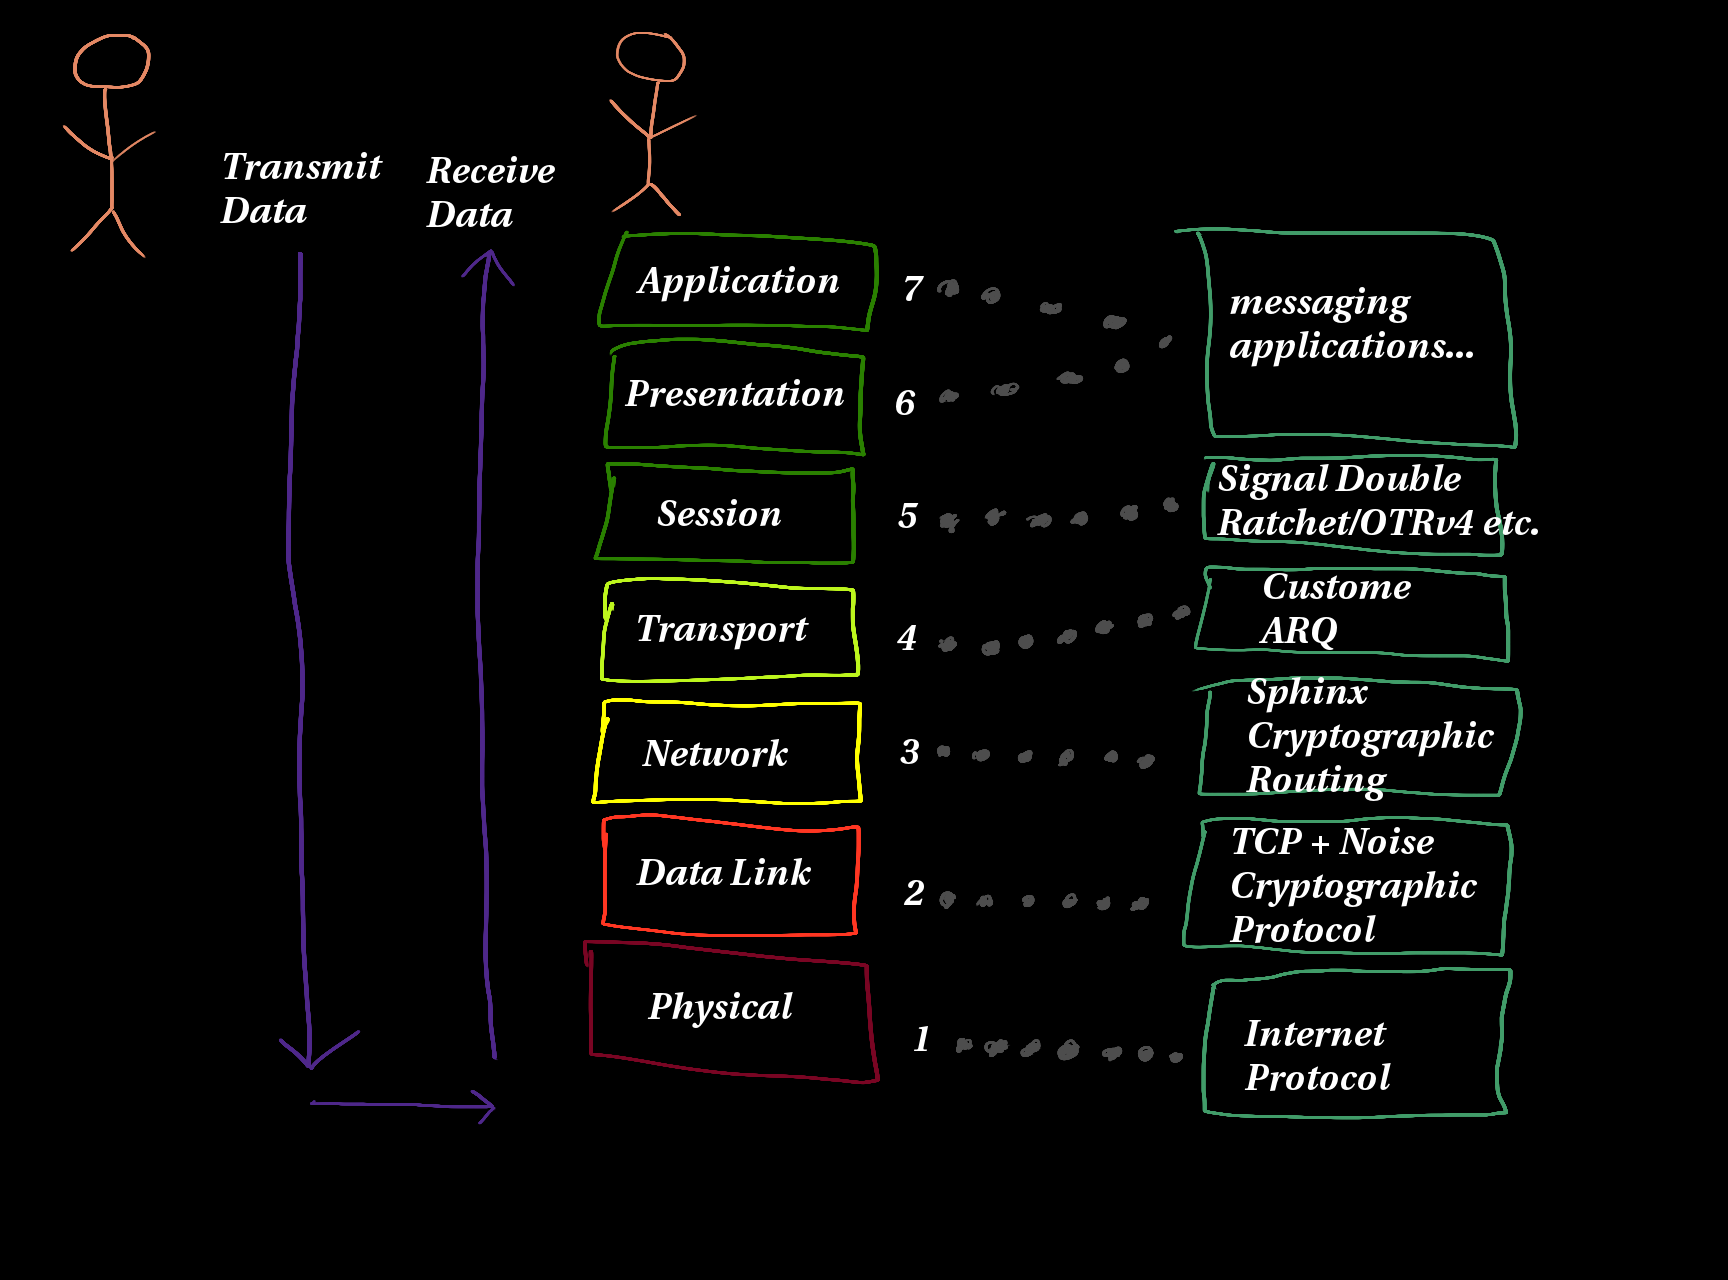
\includegraphics[scale=.19]{pics/osi_model}
\end{center}
\end{frame}

\begin{frame}
\begin{center}
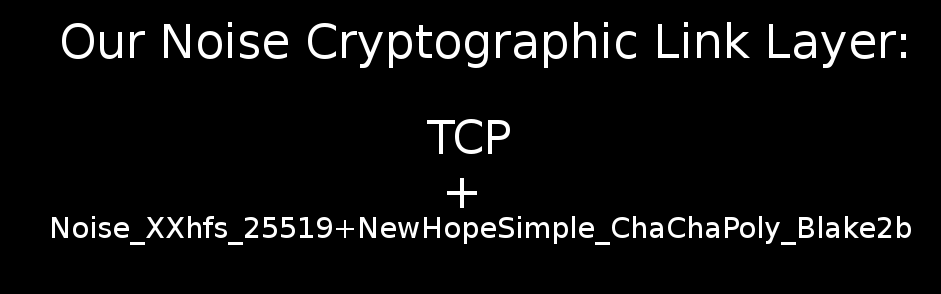
\includegraphics[scale=.33]{pics/noise_link_layer}
\end{center}
\end{frame}

\begin{frame}
\begin{center}
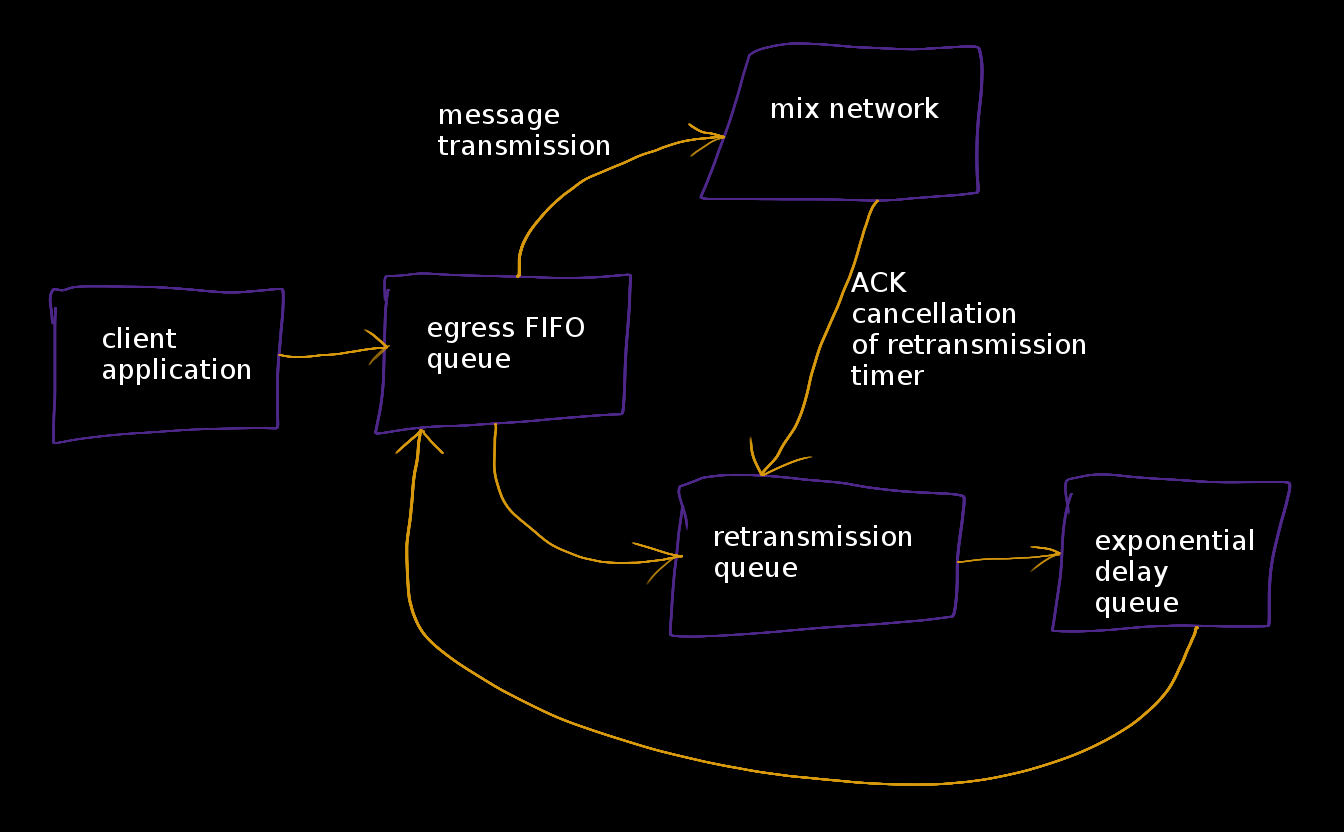
\includegraphics[scale=.24]{pics/client_aqms}
\end{center}
\end{frame}

\begin{frame}
\begin{center}
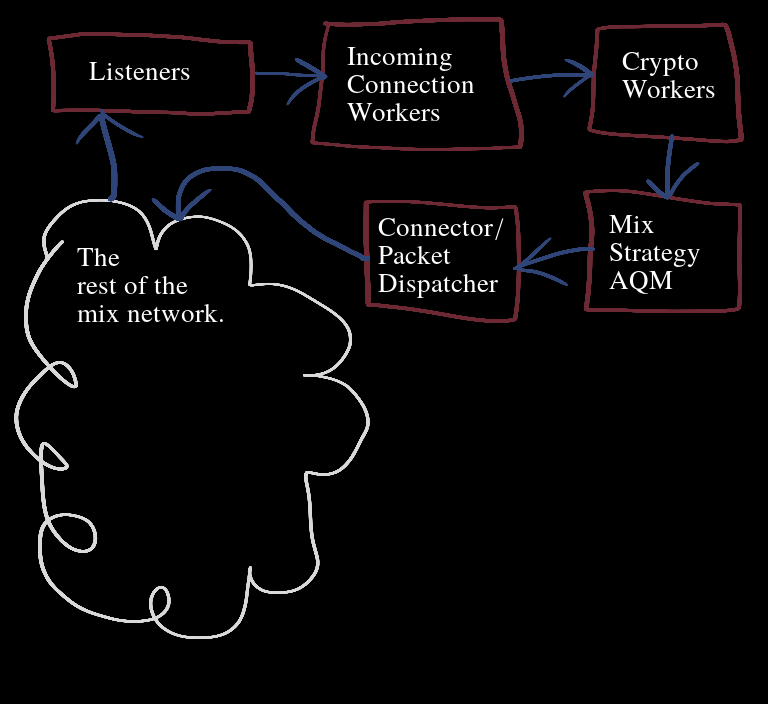
\includegraphics[scale=.33]{pics/mix_aqm_pipeline1}
\end{center}
\end{frame}

\begin{frame}
\begin{center}
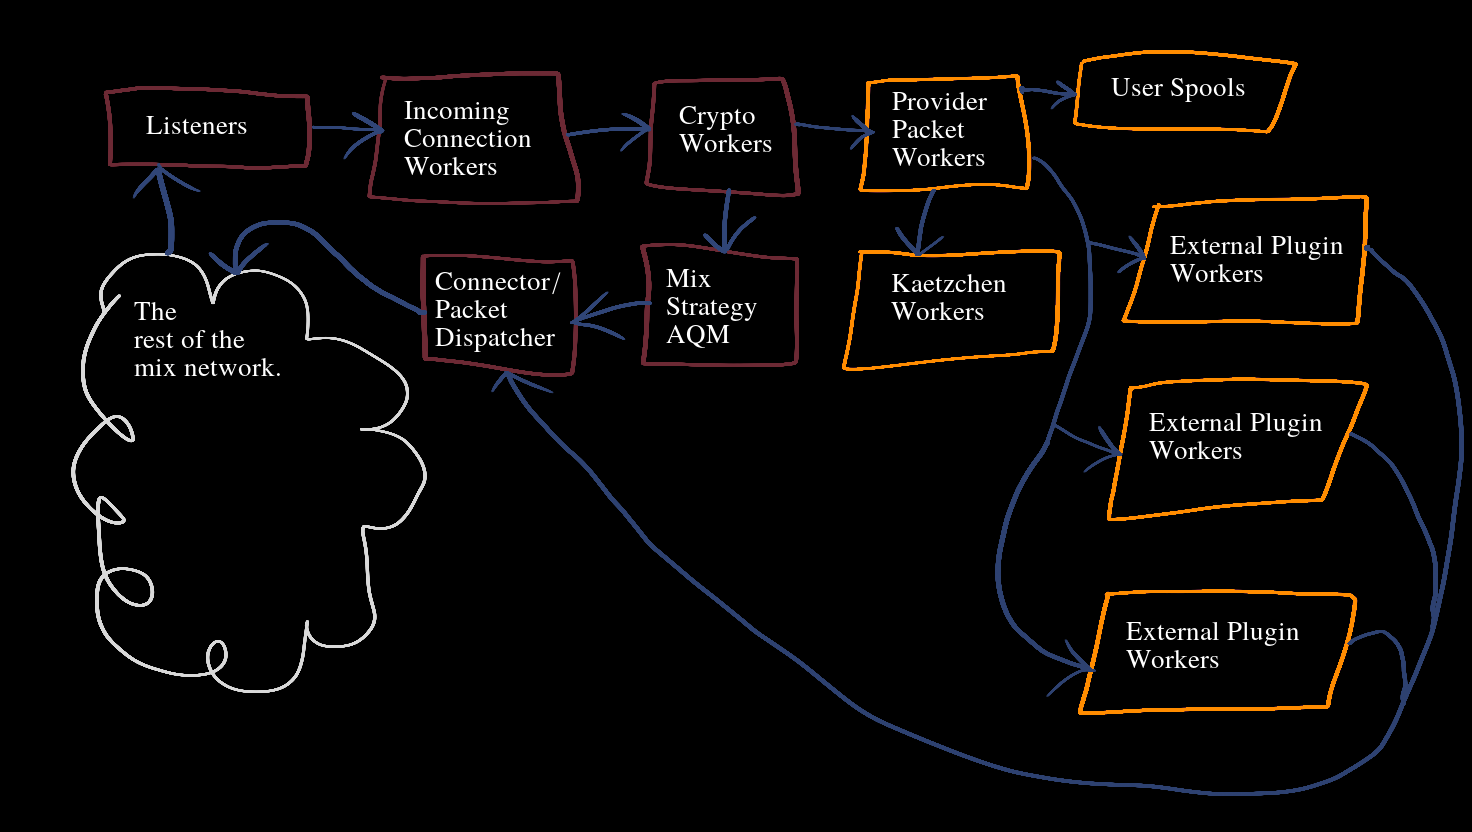
\includegraphics[scale=.22]{pics/mix_aqm_pipeline2}
\end{center}
\end{frame}


\begin{frame}
\begin{center}
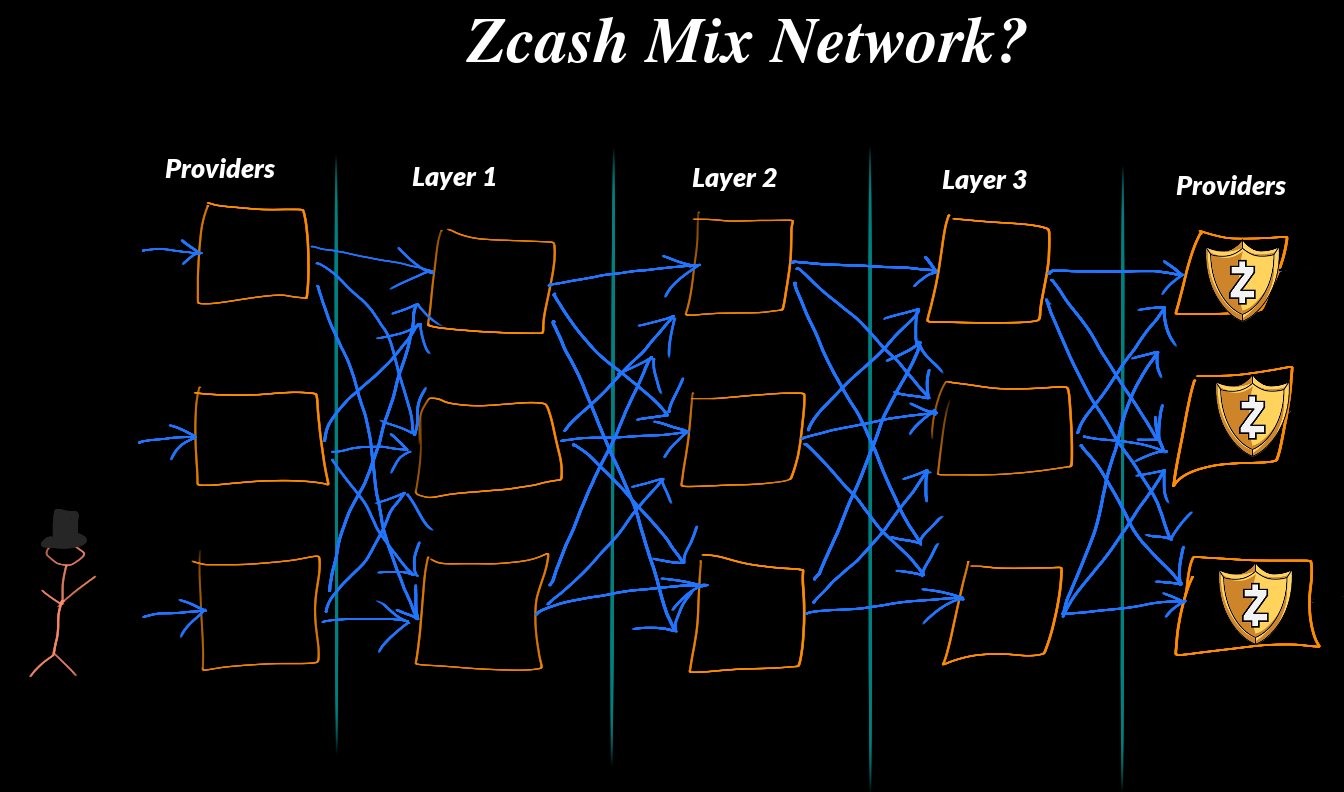
\includegraphics[scale=.24]{pics/zcash_mixnet}
\end{center}
\end{frame}


\begin{frame}{The Katzenpost Free Software Project}
  
\includegraphics[scale=0.25]{pics/katzenpost}
  \newline
  \newline
  Website:
  \newline
  https://katzenpost.mixnetworks.org/
  \newline
  \newline
  Github:
  \newline
  https://github.com/katzenpost/
  \newline
  \newline
  IRC: \#katzenpost on OFTC
  \vspace{5mm}
  \begin{itemize}
  \item Questions? Contact me: dawuud@riseup.net
  \item Follow me on twitter: @david415
  \end{itemize}    
\end{frame}


\end{document}
